 \section{Prototype work}
For this sprint we created a few new prototypes as well as refactored some of the older designs. 
Most of the new prototypes were created based on the feedback from the usability test, mentioned in \autoref{usability-test-sprint-3}.

\subsection{Choice board}
When adding an activity, it should be possible to create a choice board of multiple activities. 
As seen on \autoref{subfig:choiceboard_1}, there is a button to add a choice board on the show activity screen. 
On \autoref{subfig:choiceboard_2} the guardian can add more activities to the choice board.
\begin{figure}[H]
    \begin{subfigure}{0.5\textwidth}
    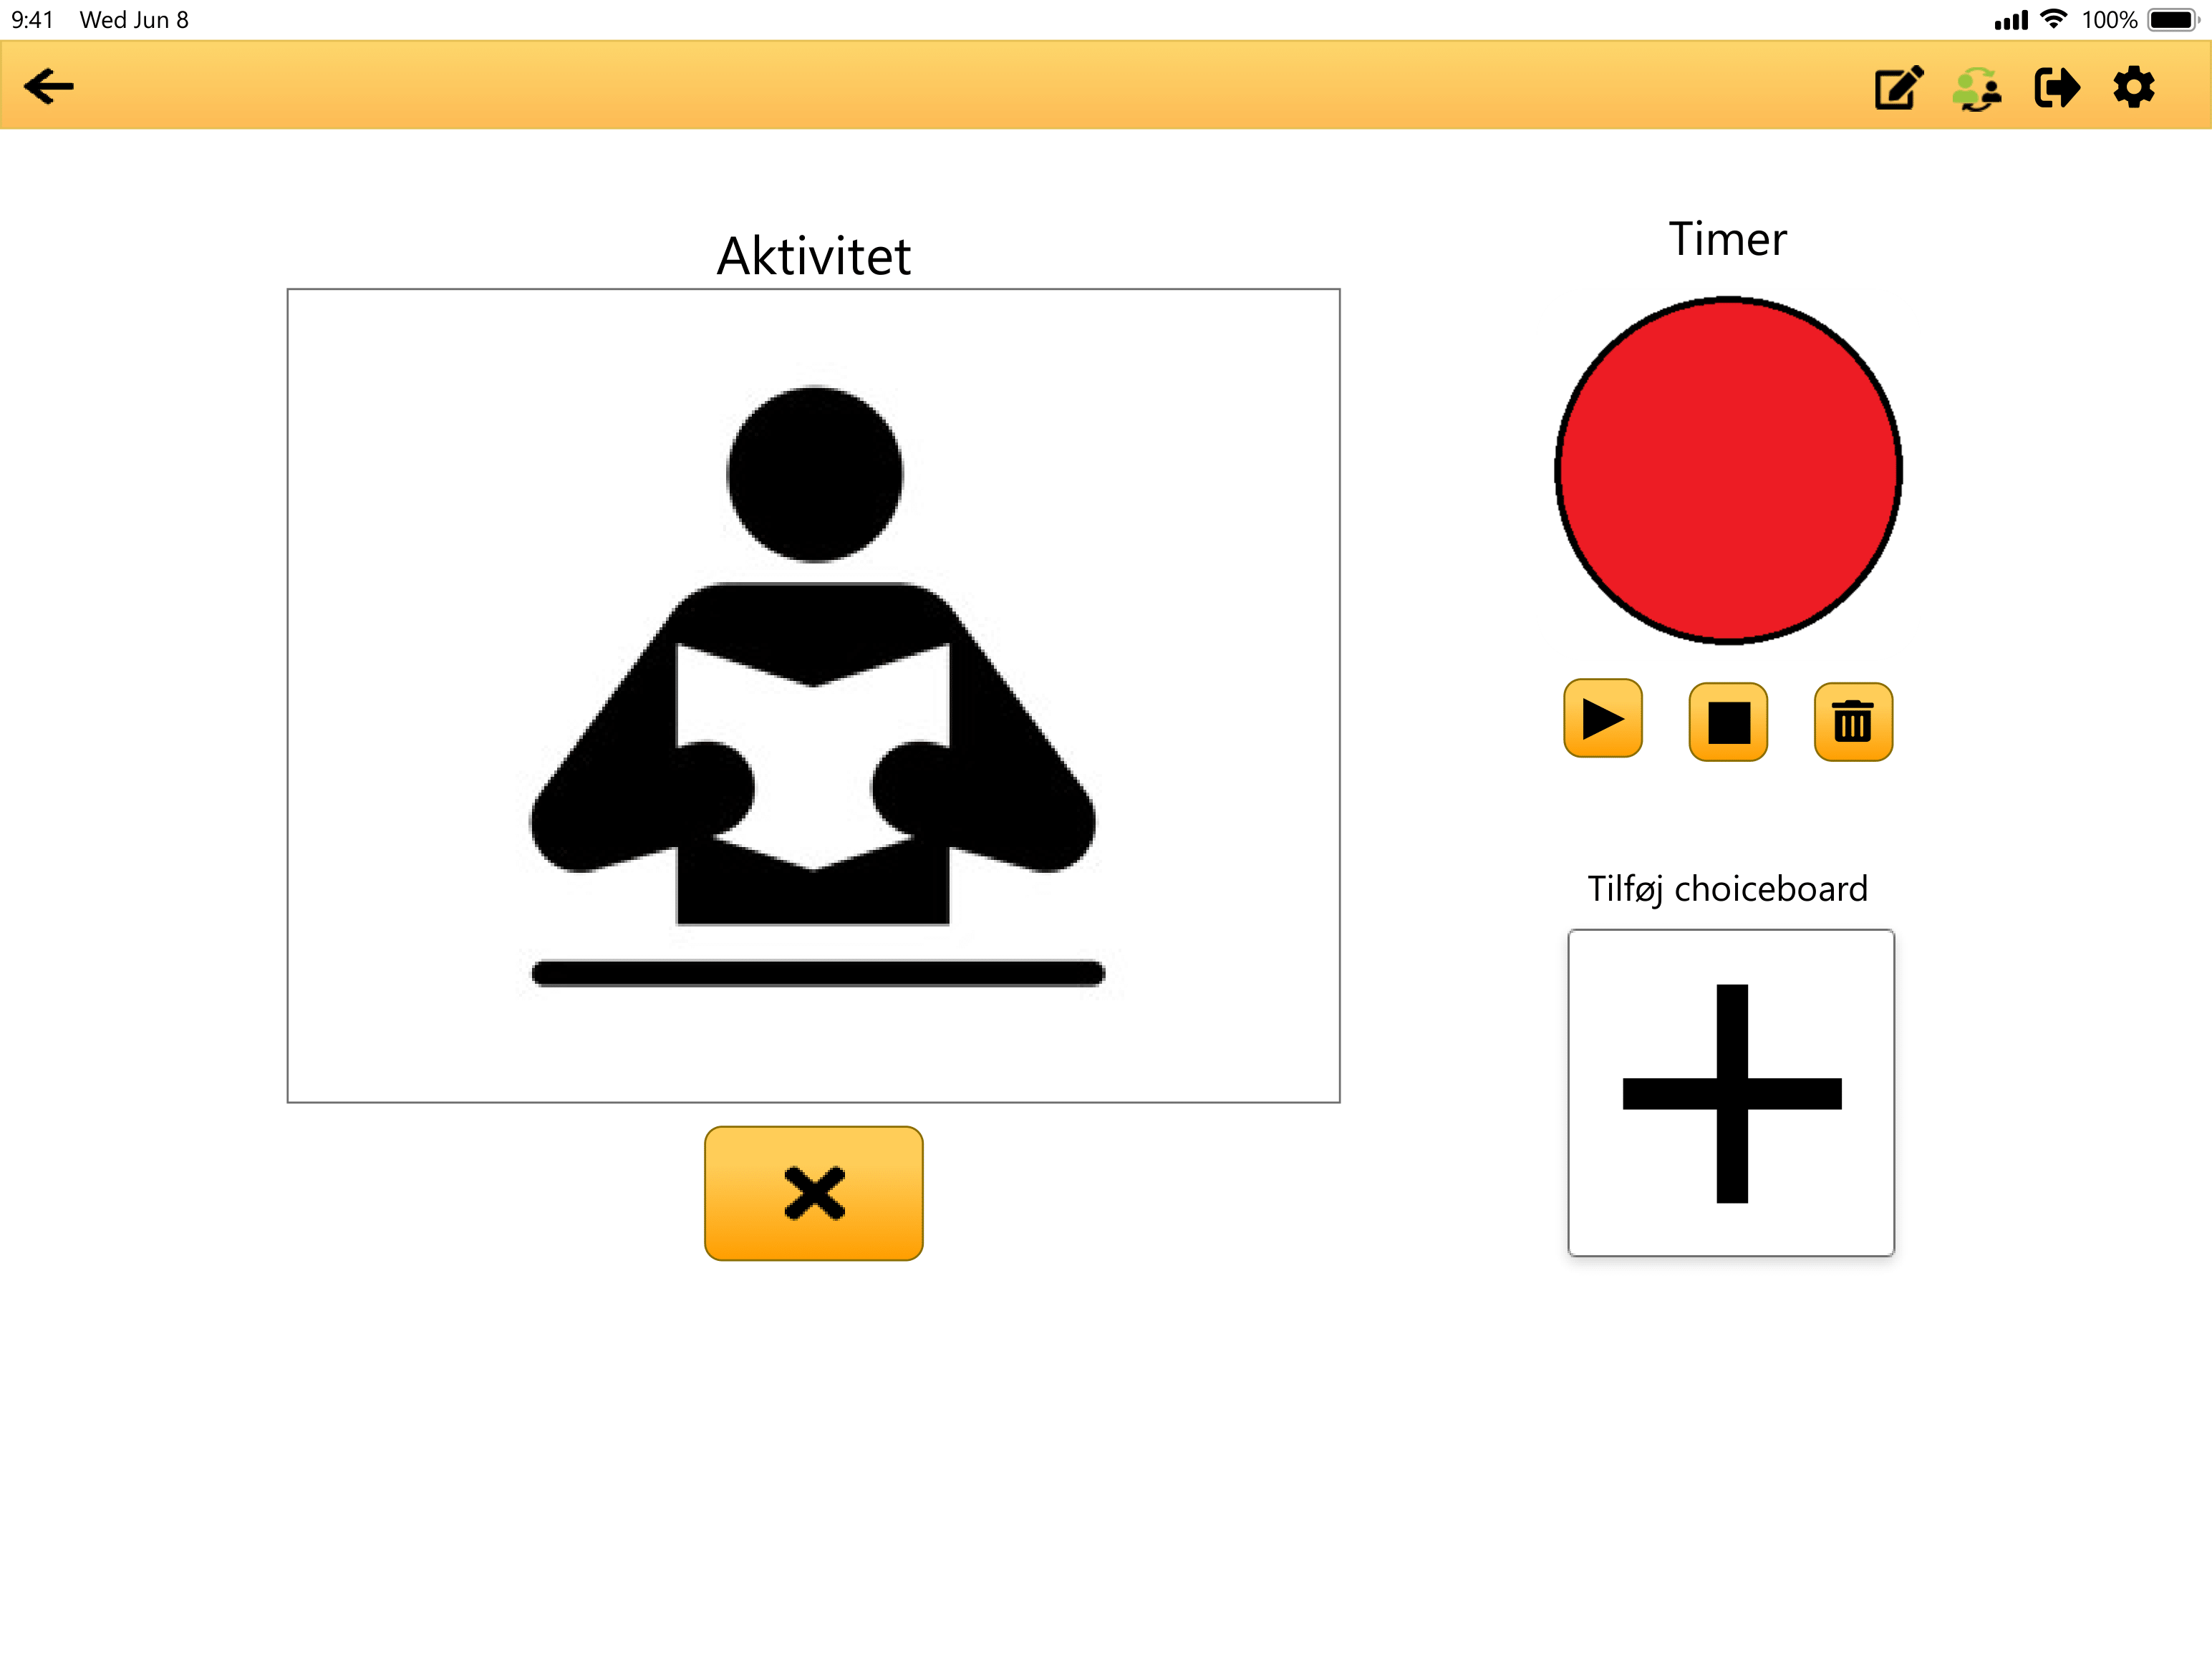
\includegraphics[width=1\linewidth, height=5cm]{choiceboard_1.png}
    \caption{Adding choice board to an activity}
    \label{subfig:choiceboard_1}
    \end{subfigure}
    \begin{subfigure}{0.5\textwidth}
    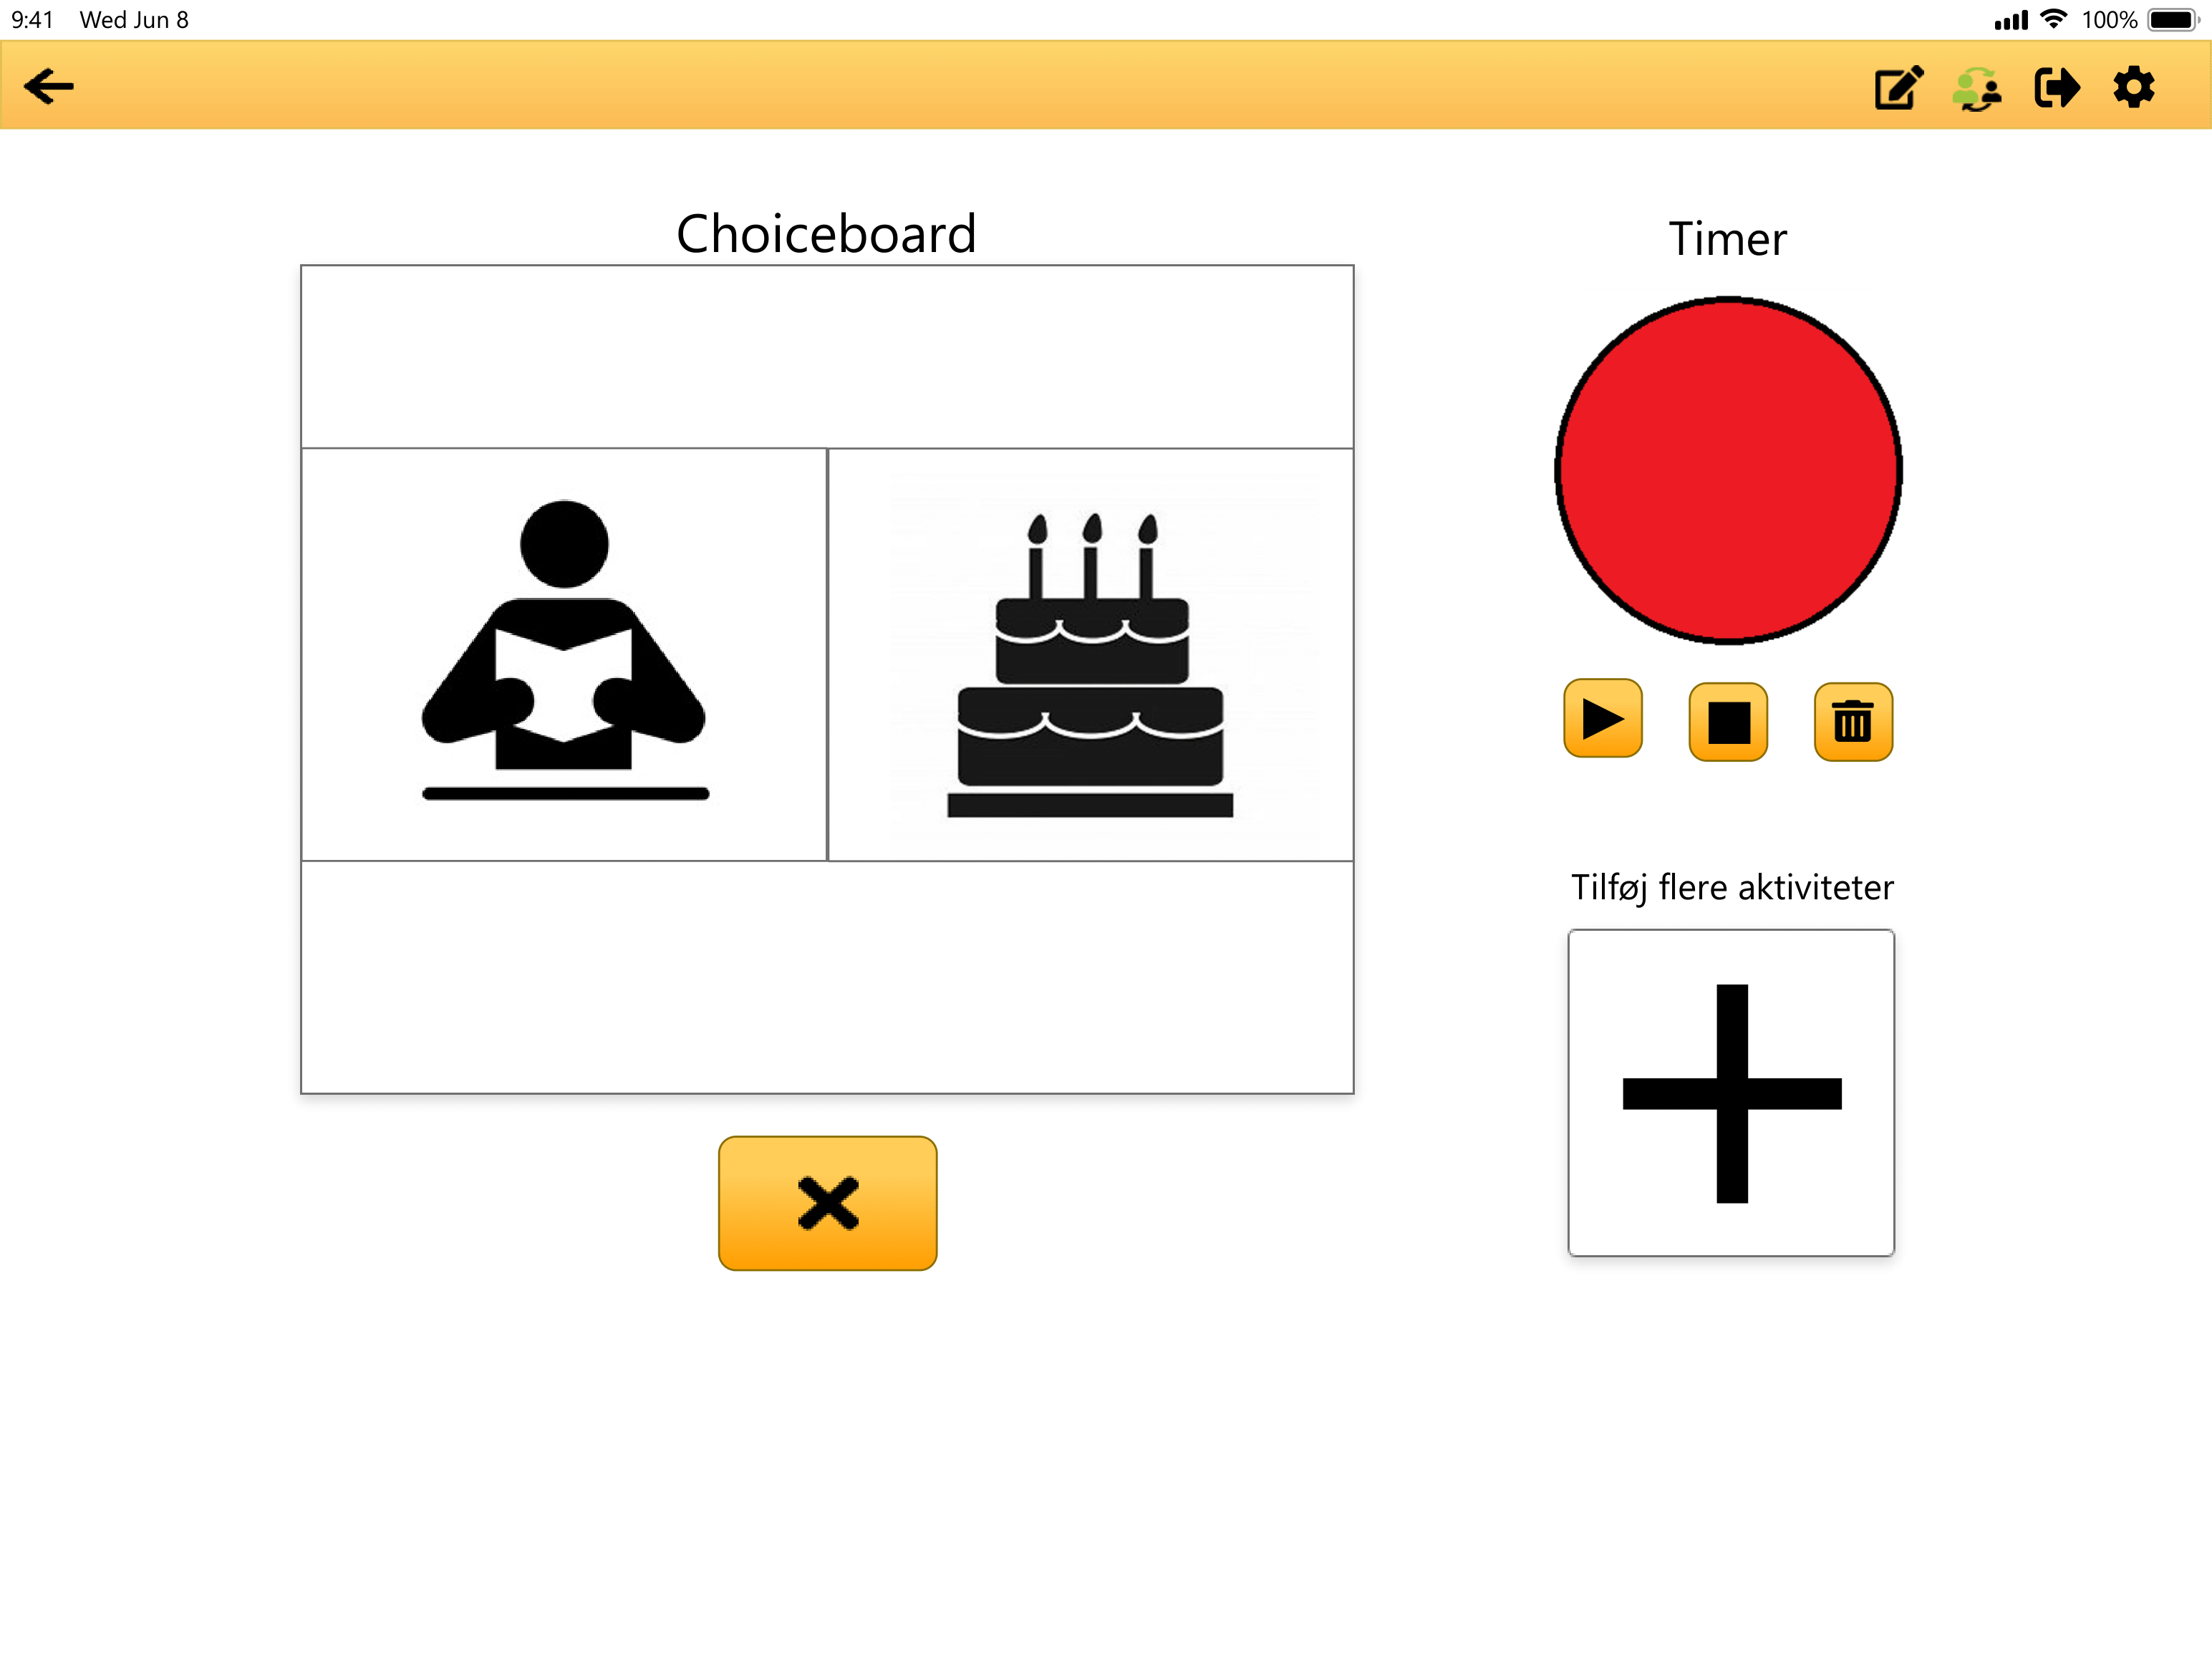
\includegraphics[width=1\linewidth, height=5cm]{choiceboard_2.png}
    \caption{Adding more activities to a choice board}
    \label{subfig:choiceboard_2}
    \end{subfigure} 
    \caption{Prototypes for adding a choice board.}
    \label{fig:choiceboardadd}
\end{figure}
\noindent
When the choice board had been created, it should be indicated on the citizen's week plan that a choice can be made between a number of activities, as seen on \autoref{subfig:choiceboard_5}.
\autoref{subfig:choiceboard_6} shows how it would look when the citizen tapped the choice board to choose between the maximum of four activities.
\begin{figure}[H]
    \begin{subfigure}{0.5\textwidth}
    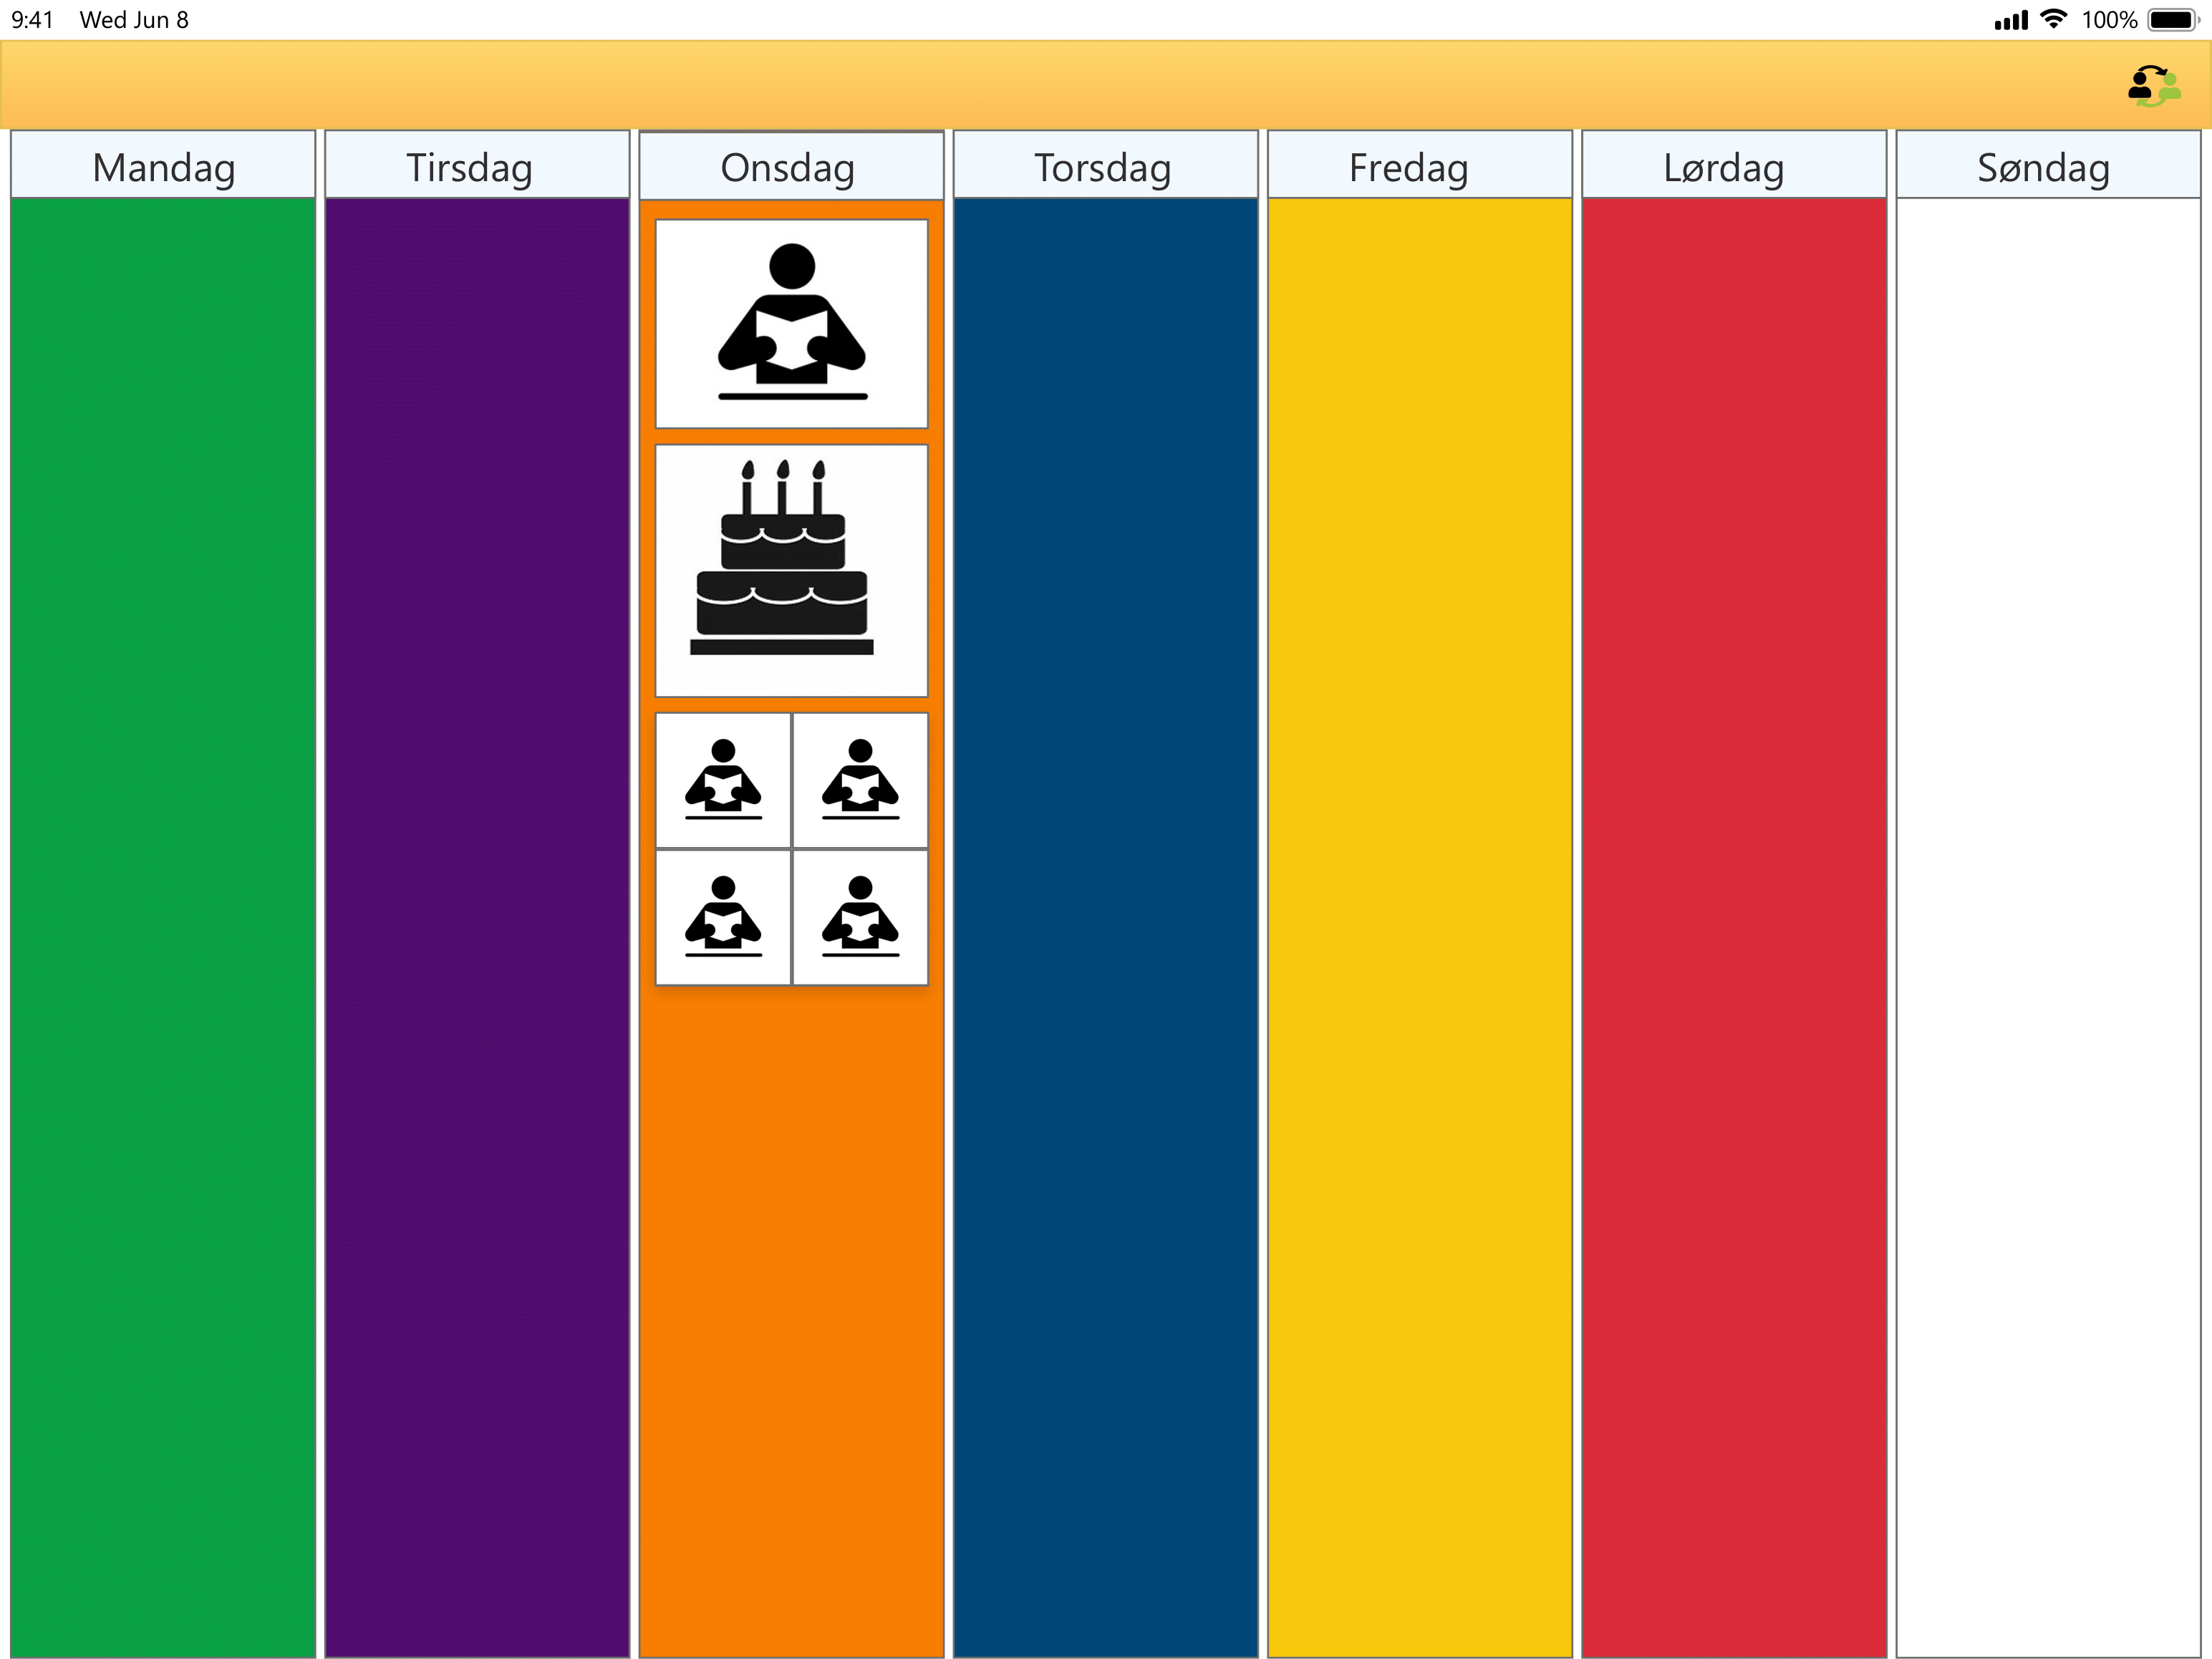
\includegraphics[width=1\linewidth, height=5cm]{choiceboard_5.png}
    \caption{Choice board as seen on the citizens view}
    \label{subfig:choiceboard_5}
    \end{subfigure}
    \begin{subfigure}{0.5\textwidth}
        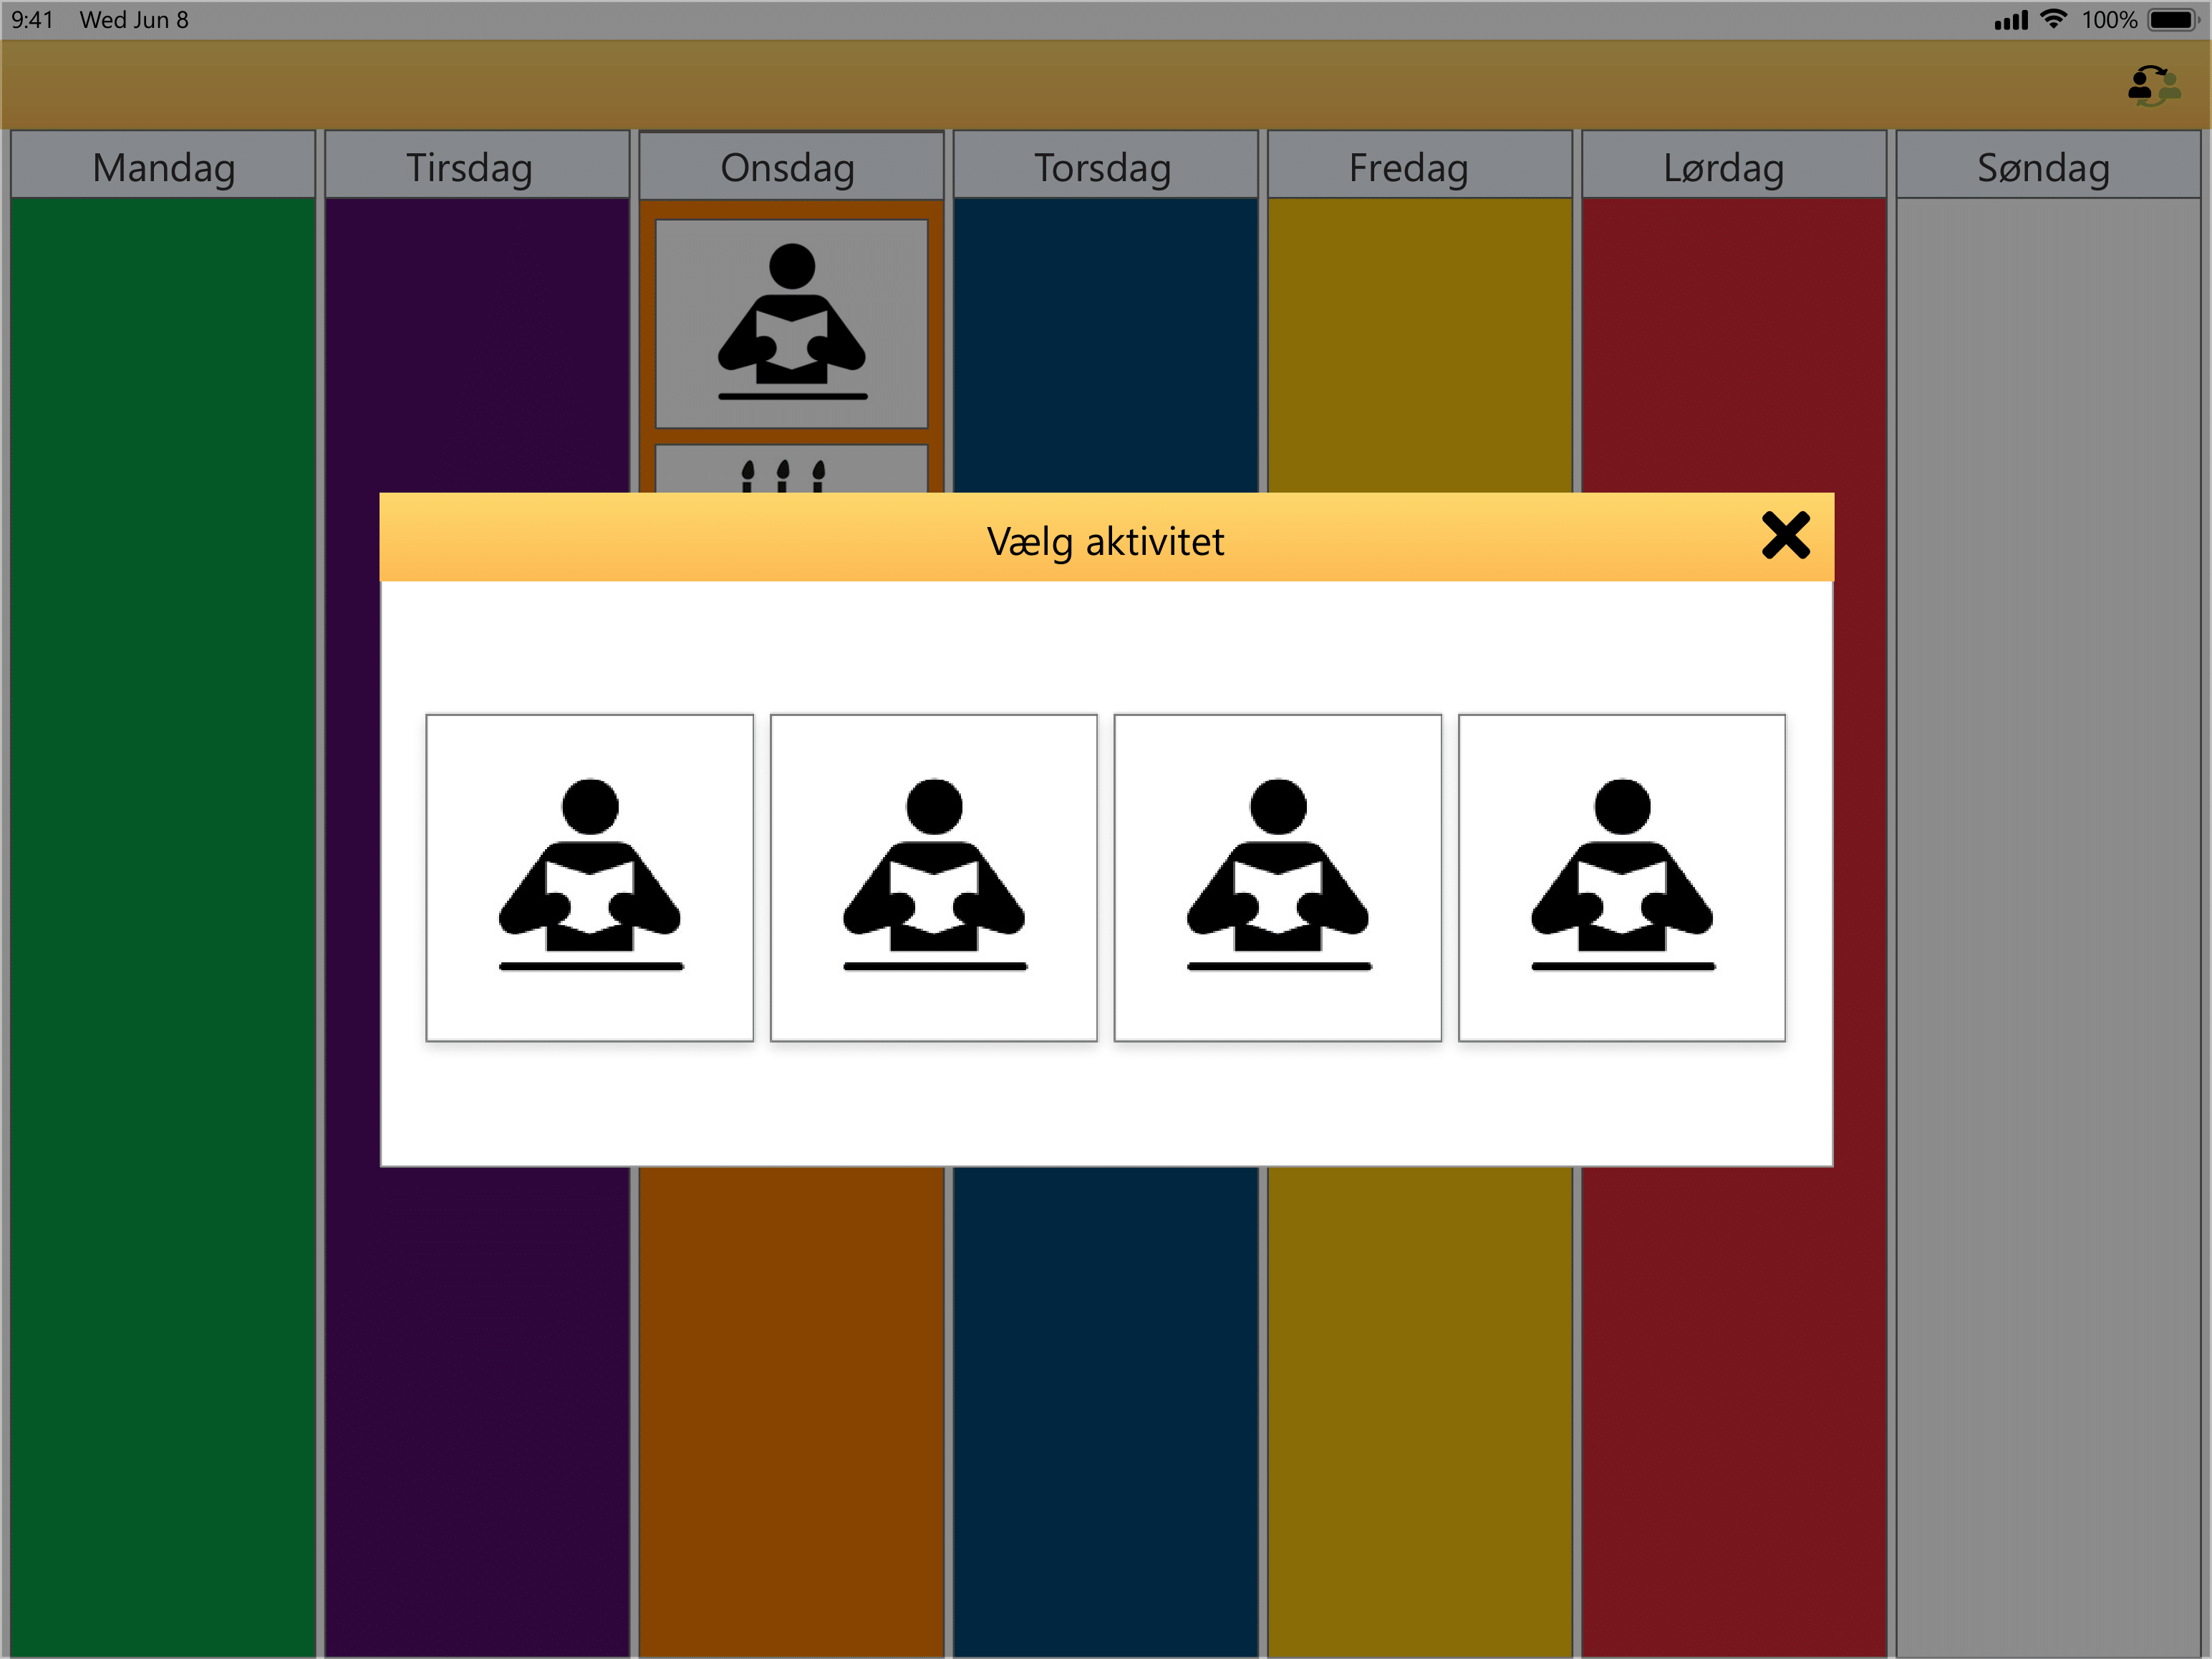
\includegraphics[width=1\linewidth, height=5cm]{choiceboard_6.png}
    \caption{Choosing an activity from choice board}
    \label{subfig:choiceboard_6}
    \end{subfigure} 
    \caption{The prototypes showing the choice boards on the week plan screen.}
    \label{fig:choiceboardcitizen}
\end{figure}

\subsection{Lock timer}
On \autoref{subfig:lock_timer_1} the prototype has a checkbox to let the guardian choose to lock the timer when it is created.
\autoref{subfig:lock_timer_3} illustrates how the locked timer has no pause button in the citizen view after the citizen has started it. 
\begin{figure}[H]
    \begin{subfigure}{0.5\textwidth}
    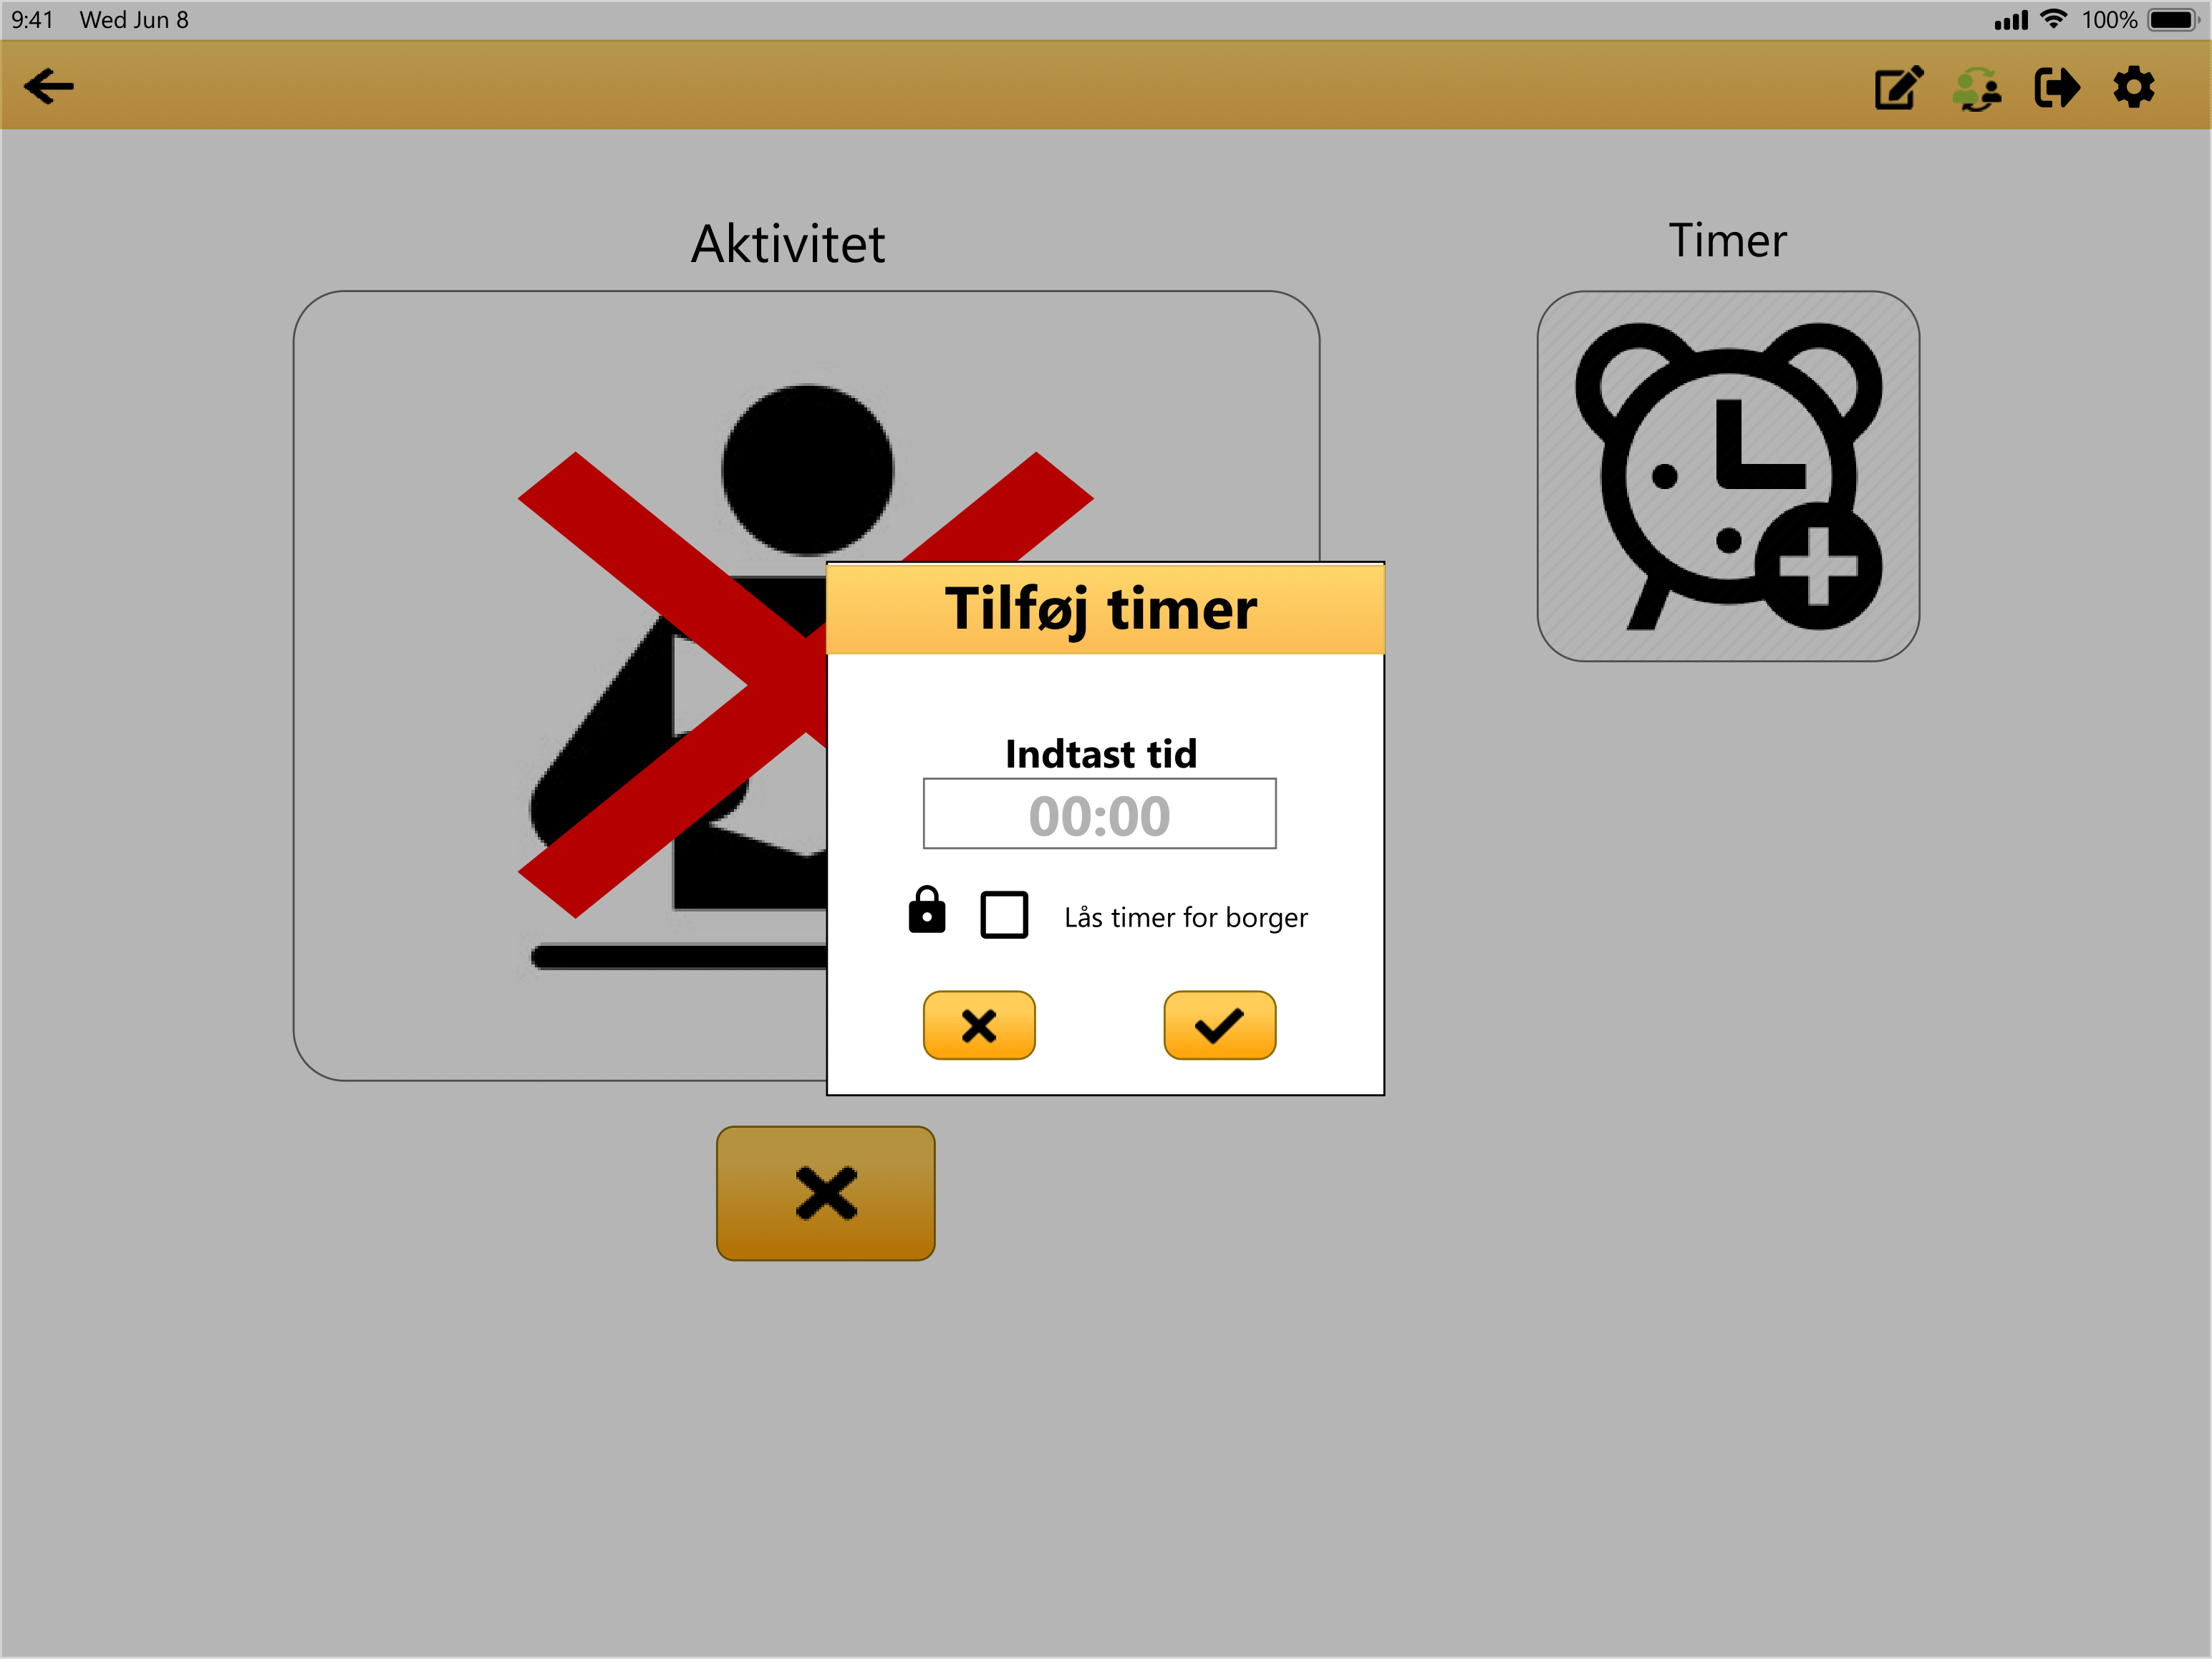
\includegraphics[width=1\linewidth, height=5cm]{lock_timer_1.png}
    \caption{Checkmark to lock timer}
    \label{subfig:lock_timer_1}
    \end{subfigure}
    \begin{subfigure}{0.5\textwidth}
        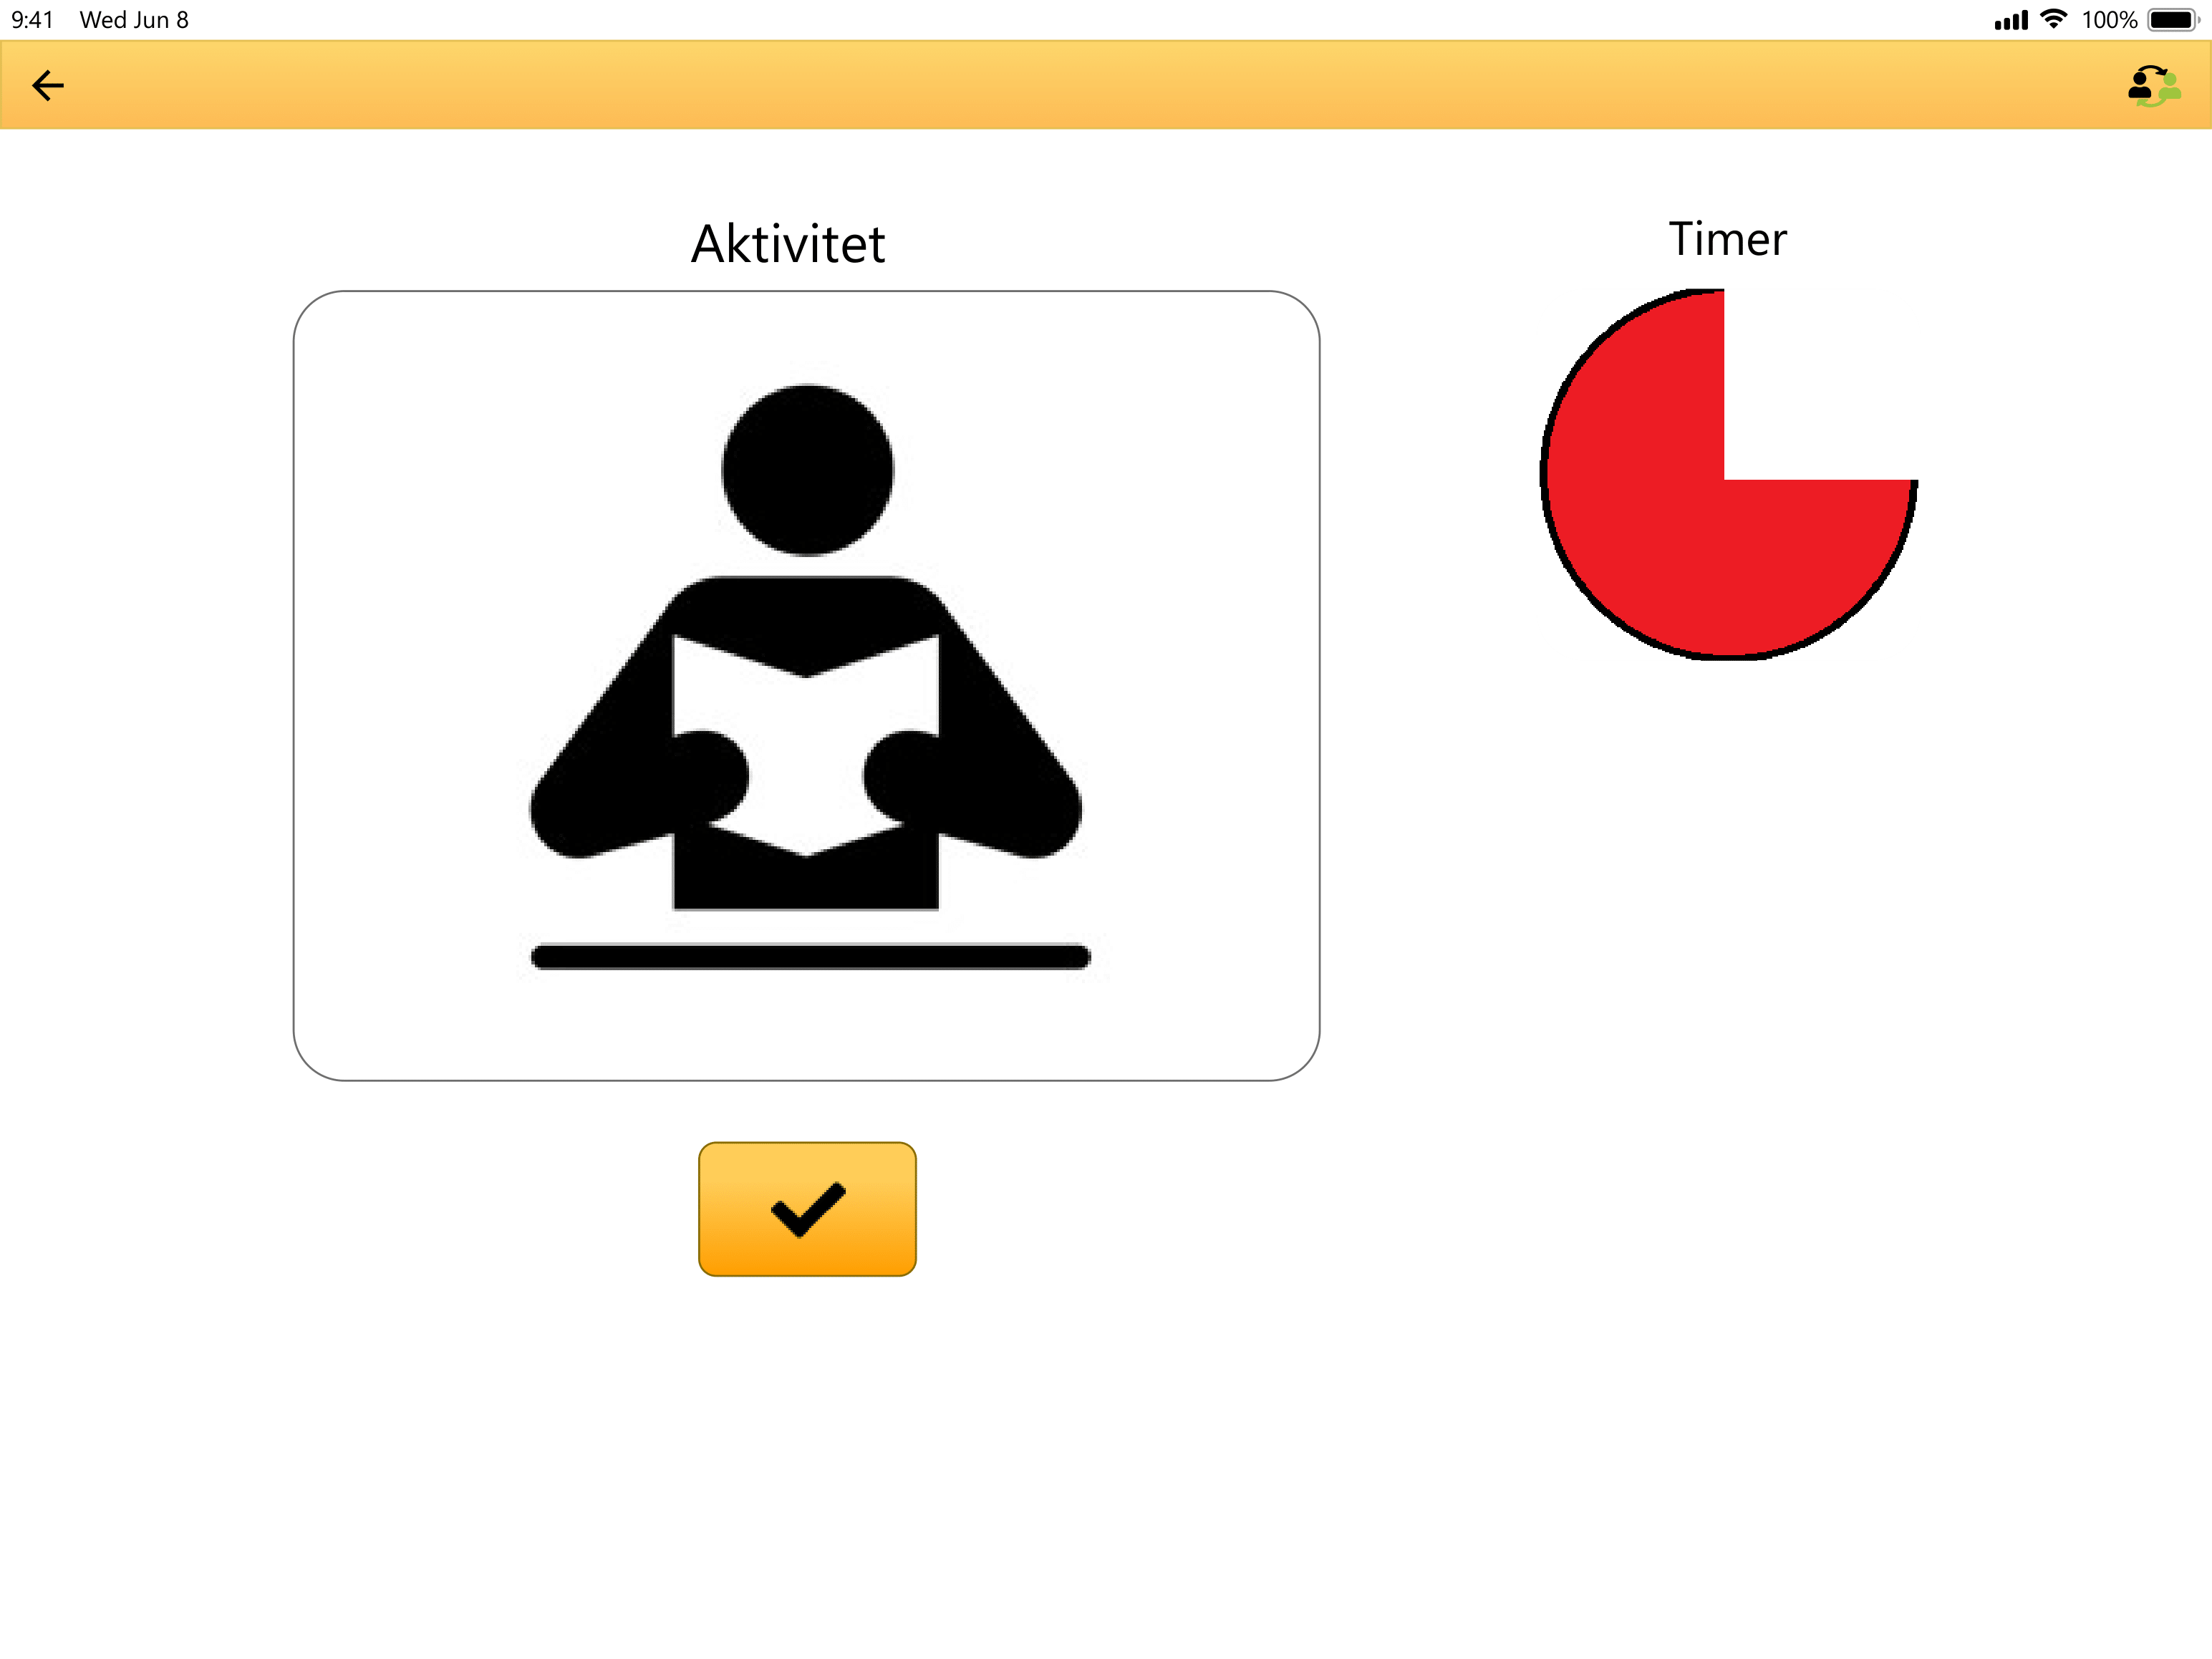
\includegraphics[width=1\linewidth, height=5cm]{lock_timer_3.png}
    \caption{No pause button for citizen on the timer}
    \label{subfig:lock_timer_3}
    \end{subfigure} 
    \caption{The prototype illustrating the functionality to lock a timer.}
    \label{fig:lock_timer}
\end{figure}

\subsection{Drag and drop activities}
We learned during the usability test in sprint 3 that it was difficult to see where the pictogram would be placed when dragging and dropping it.
Therefore, we created these prototypes that show how it could look when a pictogram is being repositioned.
\autoref{subfig:drag_n_drop_2} shows the start of a drag and drop action.
It indicates for each weekday where it can be placed. 
On \autoref{subfig:drag_n_drop_3} the positions of the existing activities on a weekday are changed when dragging an activity between two existing activities to indicate where it would be positioned.
\begin{figure}[H]
    \begin{subfigure}{0.5\textwidth}
    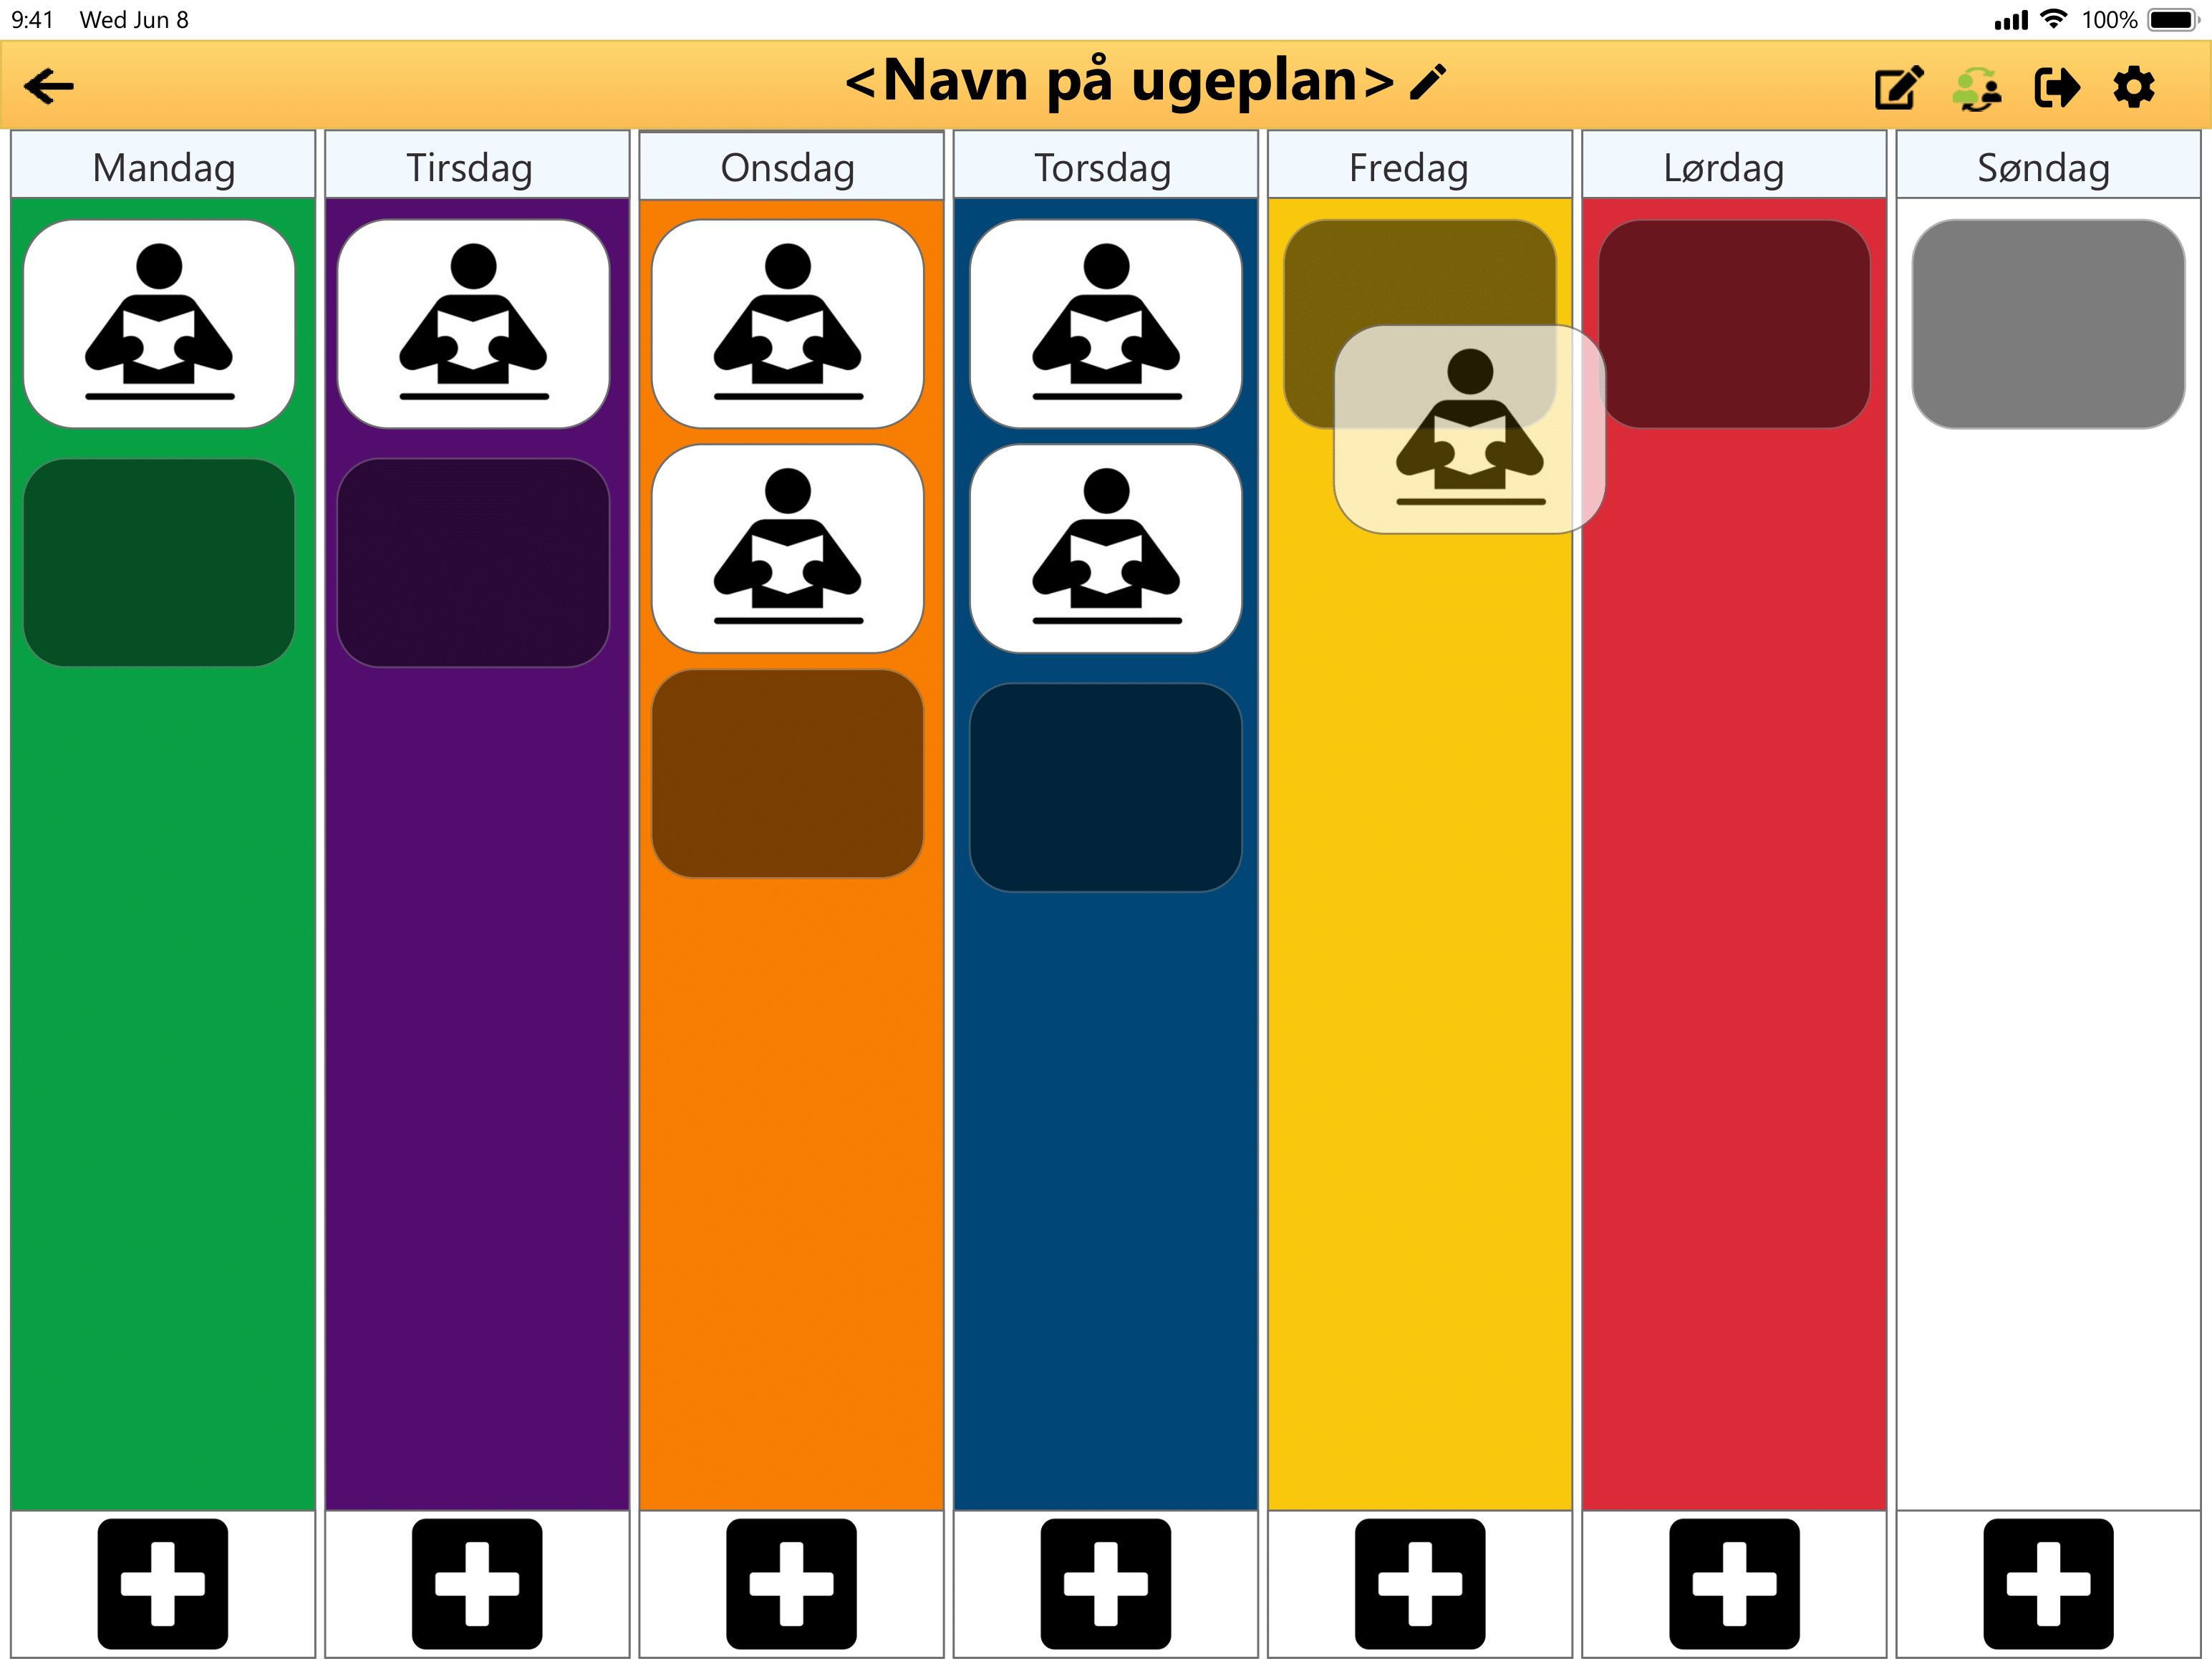
\includegraphics[width=1\linewidth, height=5cm]{drag_n_drop_2.png}
    \caption{Dragging an activity}
    \label{subfig:drag_n_drop_2}
    \end{subfigure}
    \begin{subfigure}{0.5\textwidth}
        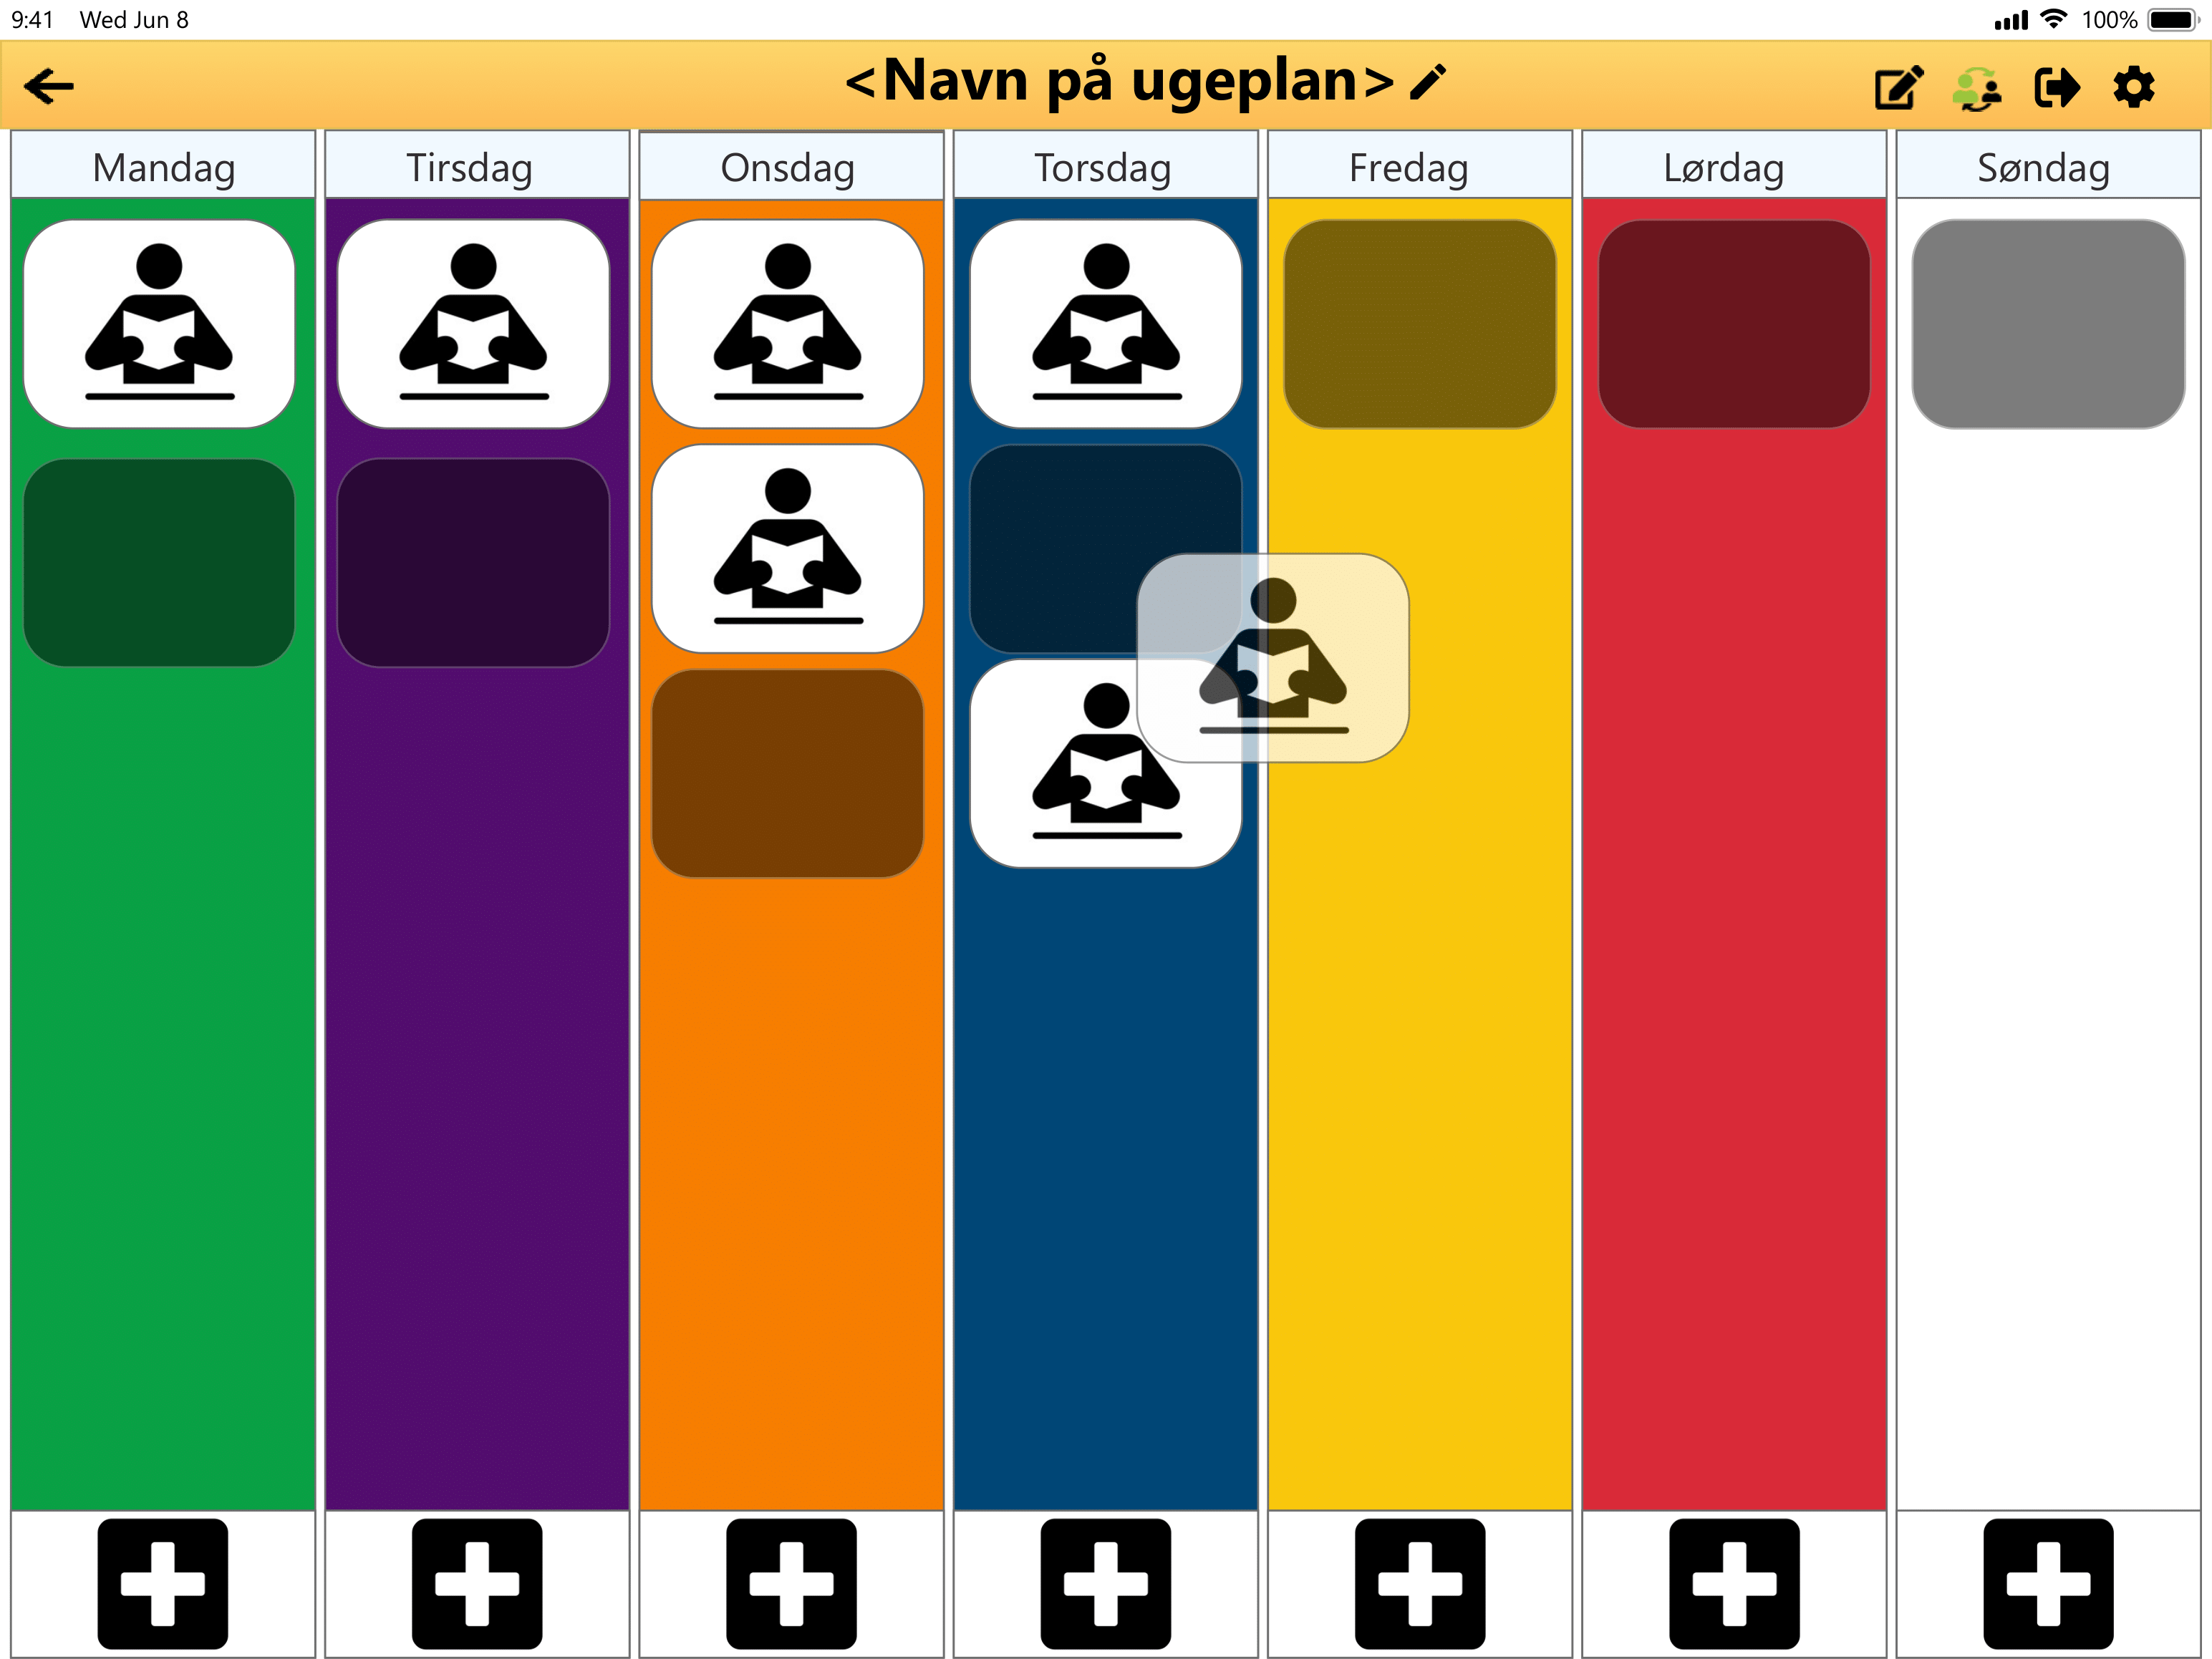
\includegraphics[width=1\linewidth, height=5cm]{drag_n_drop_3.png}
    \caption{Dragging an activity between activities}
    \label{subfig:drag_n_drop_3}
    \end{subfigure} 
    \caption{The prototypes for visualizing dragging and dropping activities.}
    \label{fig:drag_n_drop}
\end{figure}

\subsection{Adding citizens} 
The first prototype on \autoref{subfig:add_citizen_1} has an icon on the choose citizen screen that can be tapped to create a new citizen.
\autoref{subfig:add_citizen_2} shows the screen where a new citizen can be created by entering a name and adding a picture.
\begin{figure}[H]
    \begin{subfigure}{0.5\textwidth}
    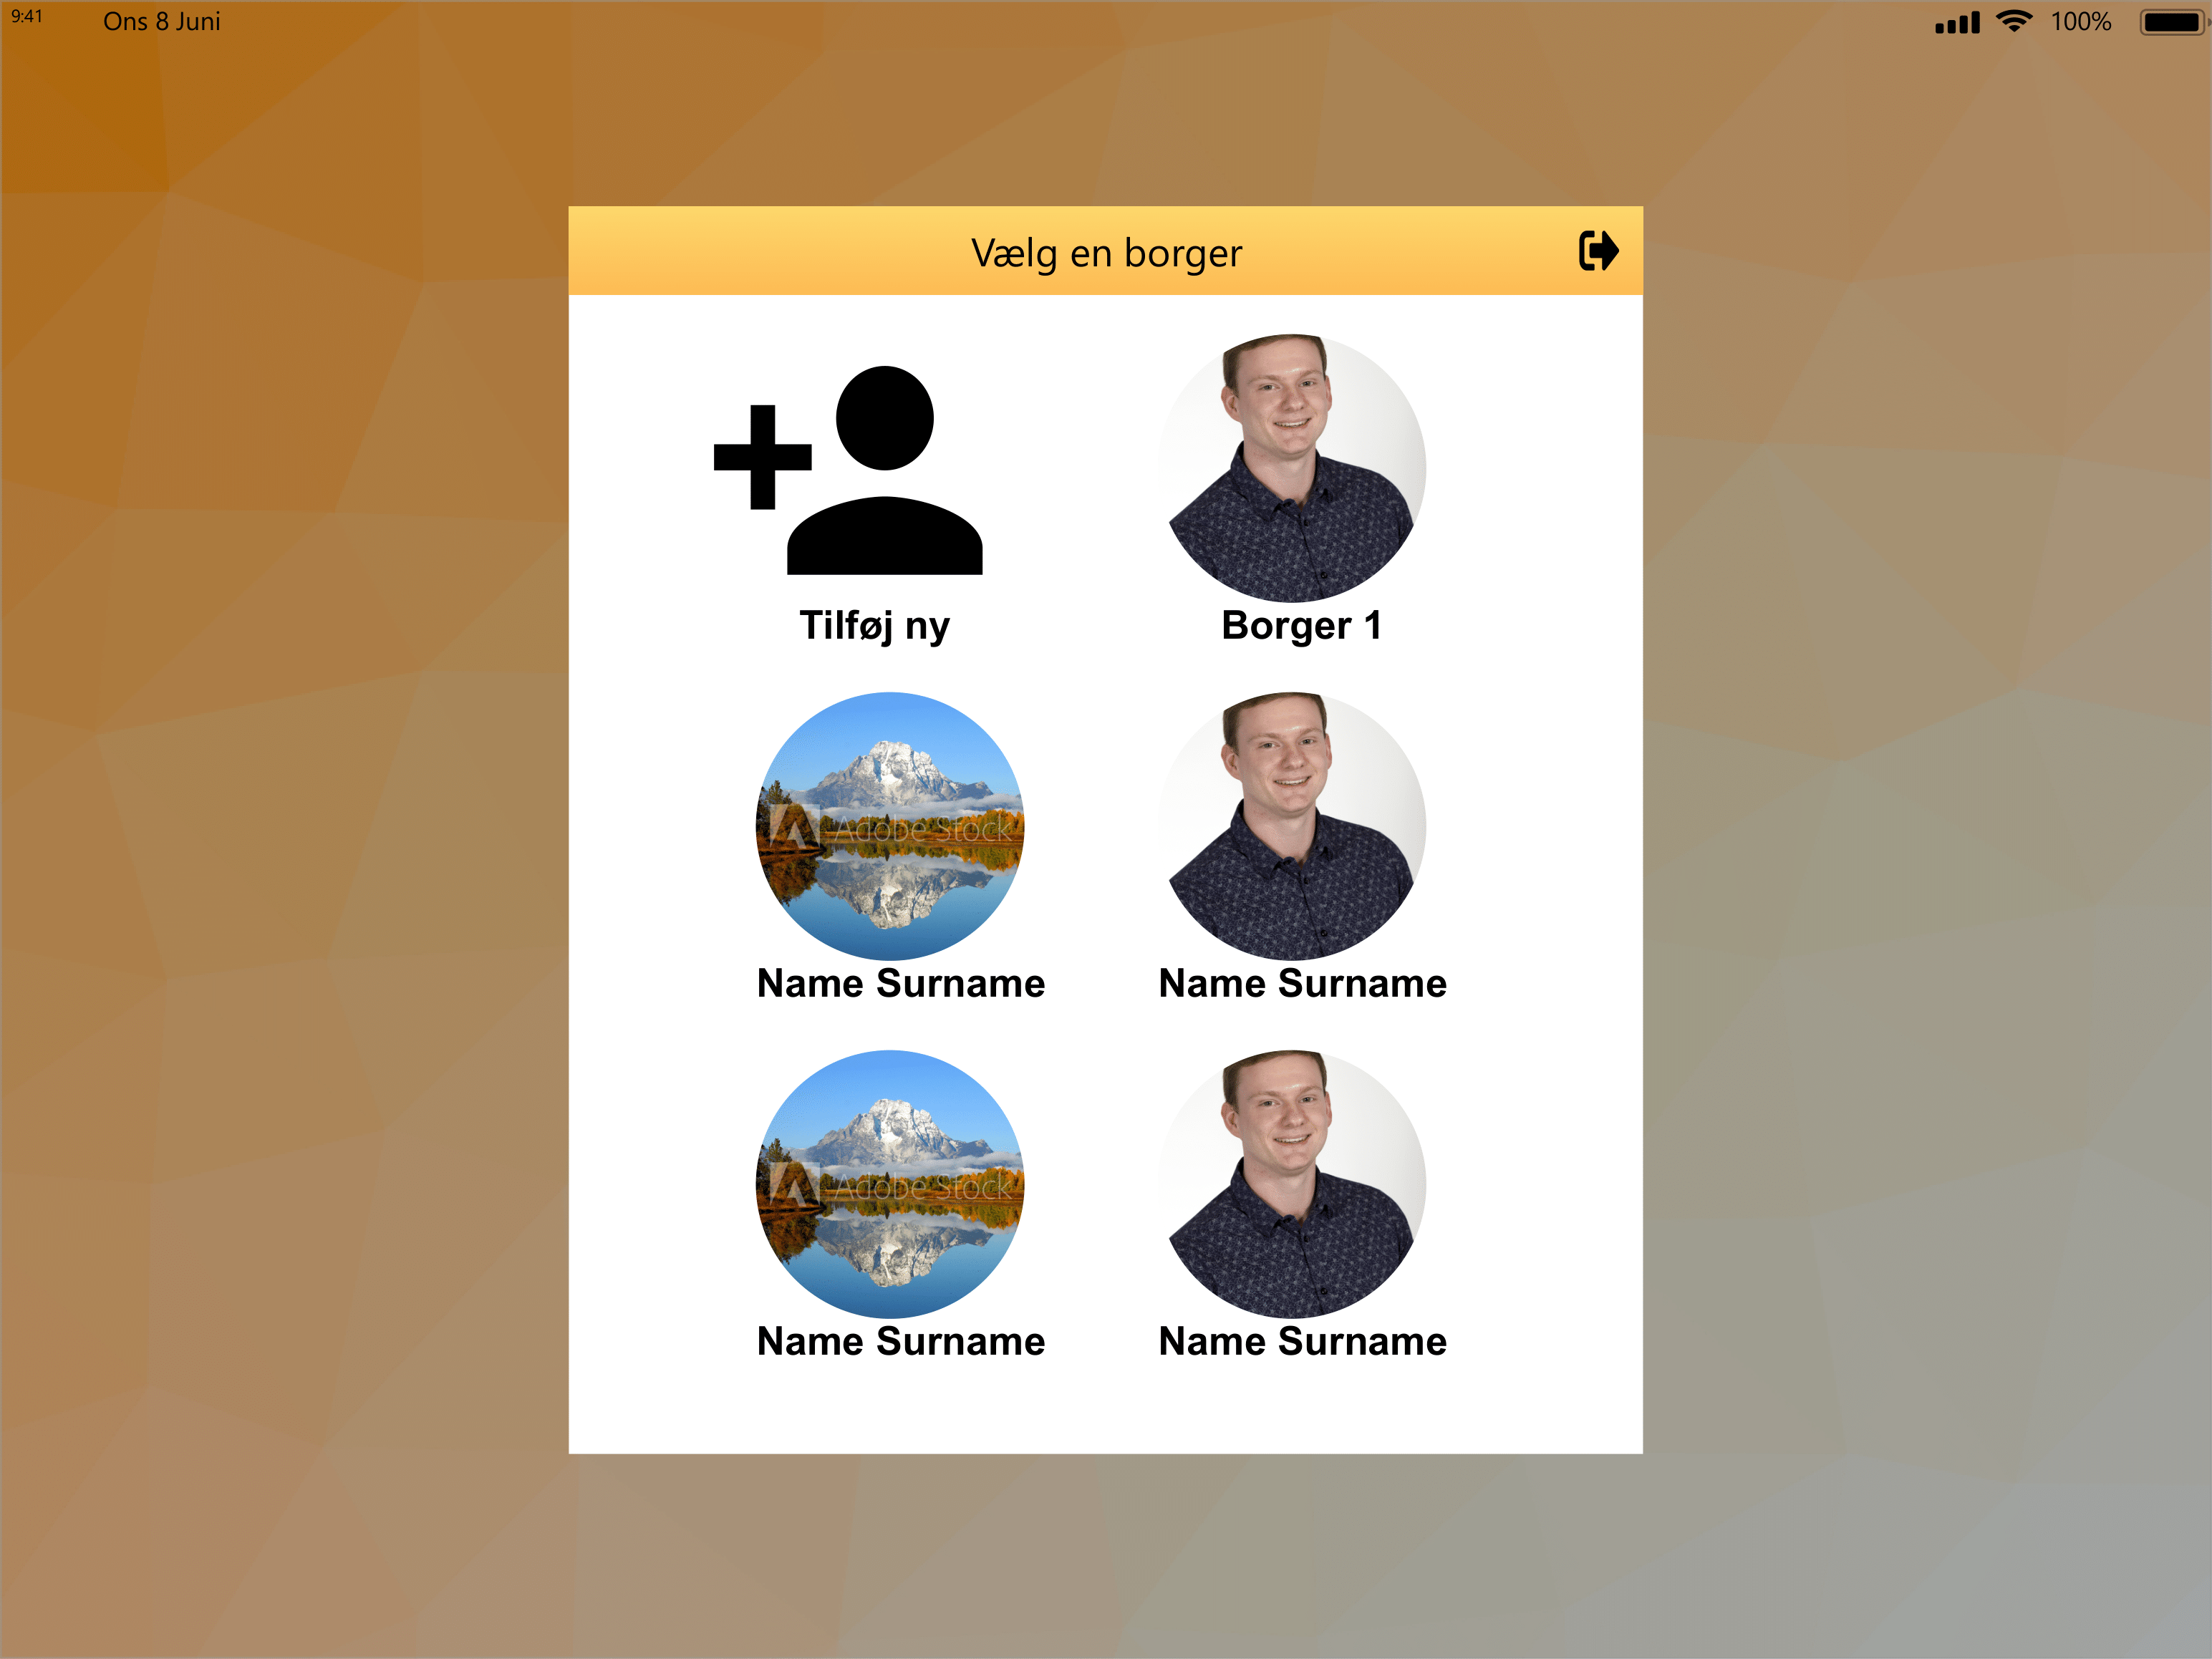
\includegraphics[width=1\linewidth, height=5cm]{add_citizen_1.png}
    \caption{Icon to add new citizen}
    \label{subfig:add_citizen_1}
    \end{subfigure}
    \begin{subfigure}{0.5\textwidth}
        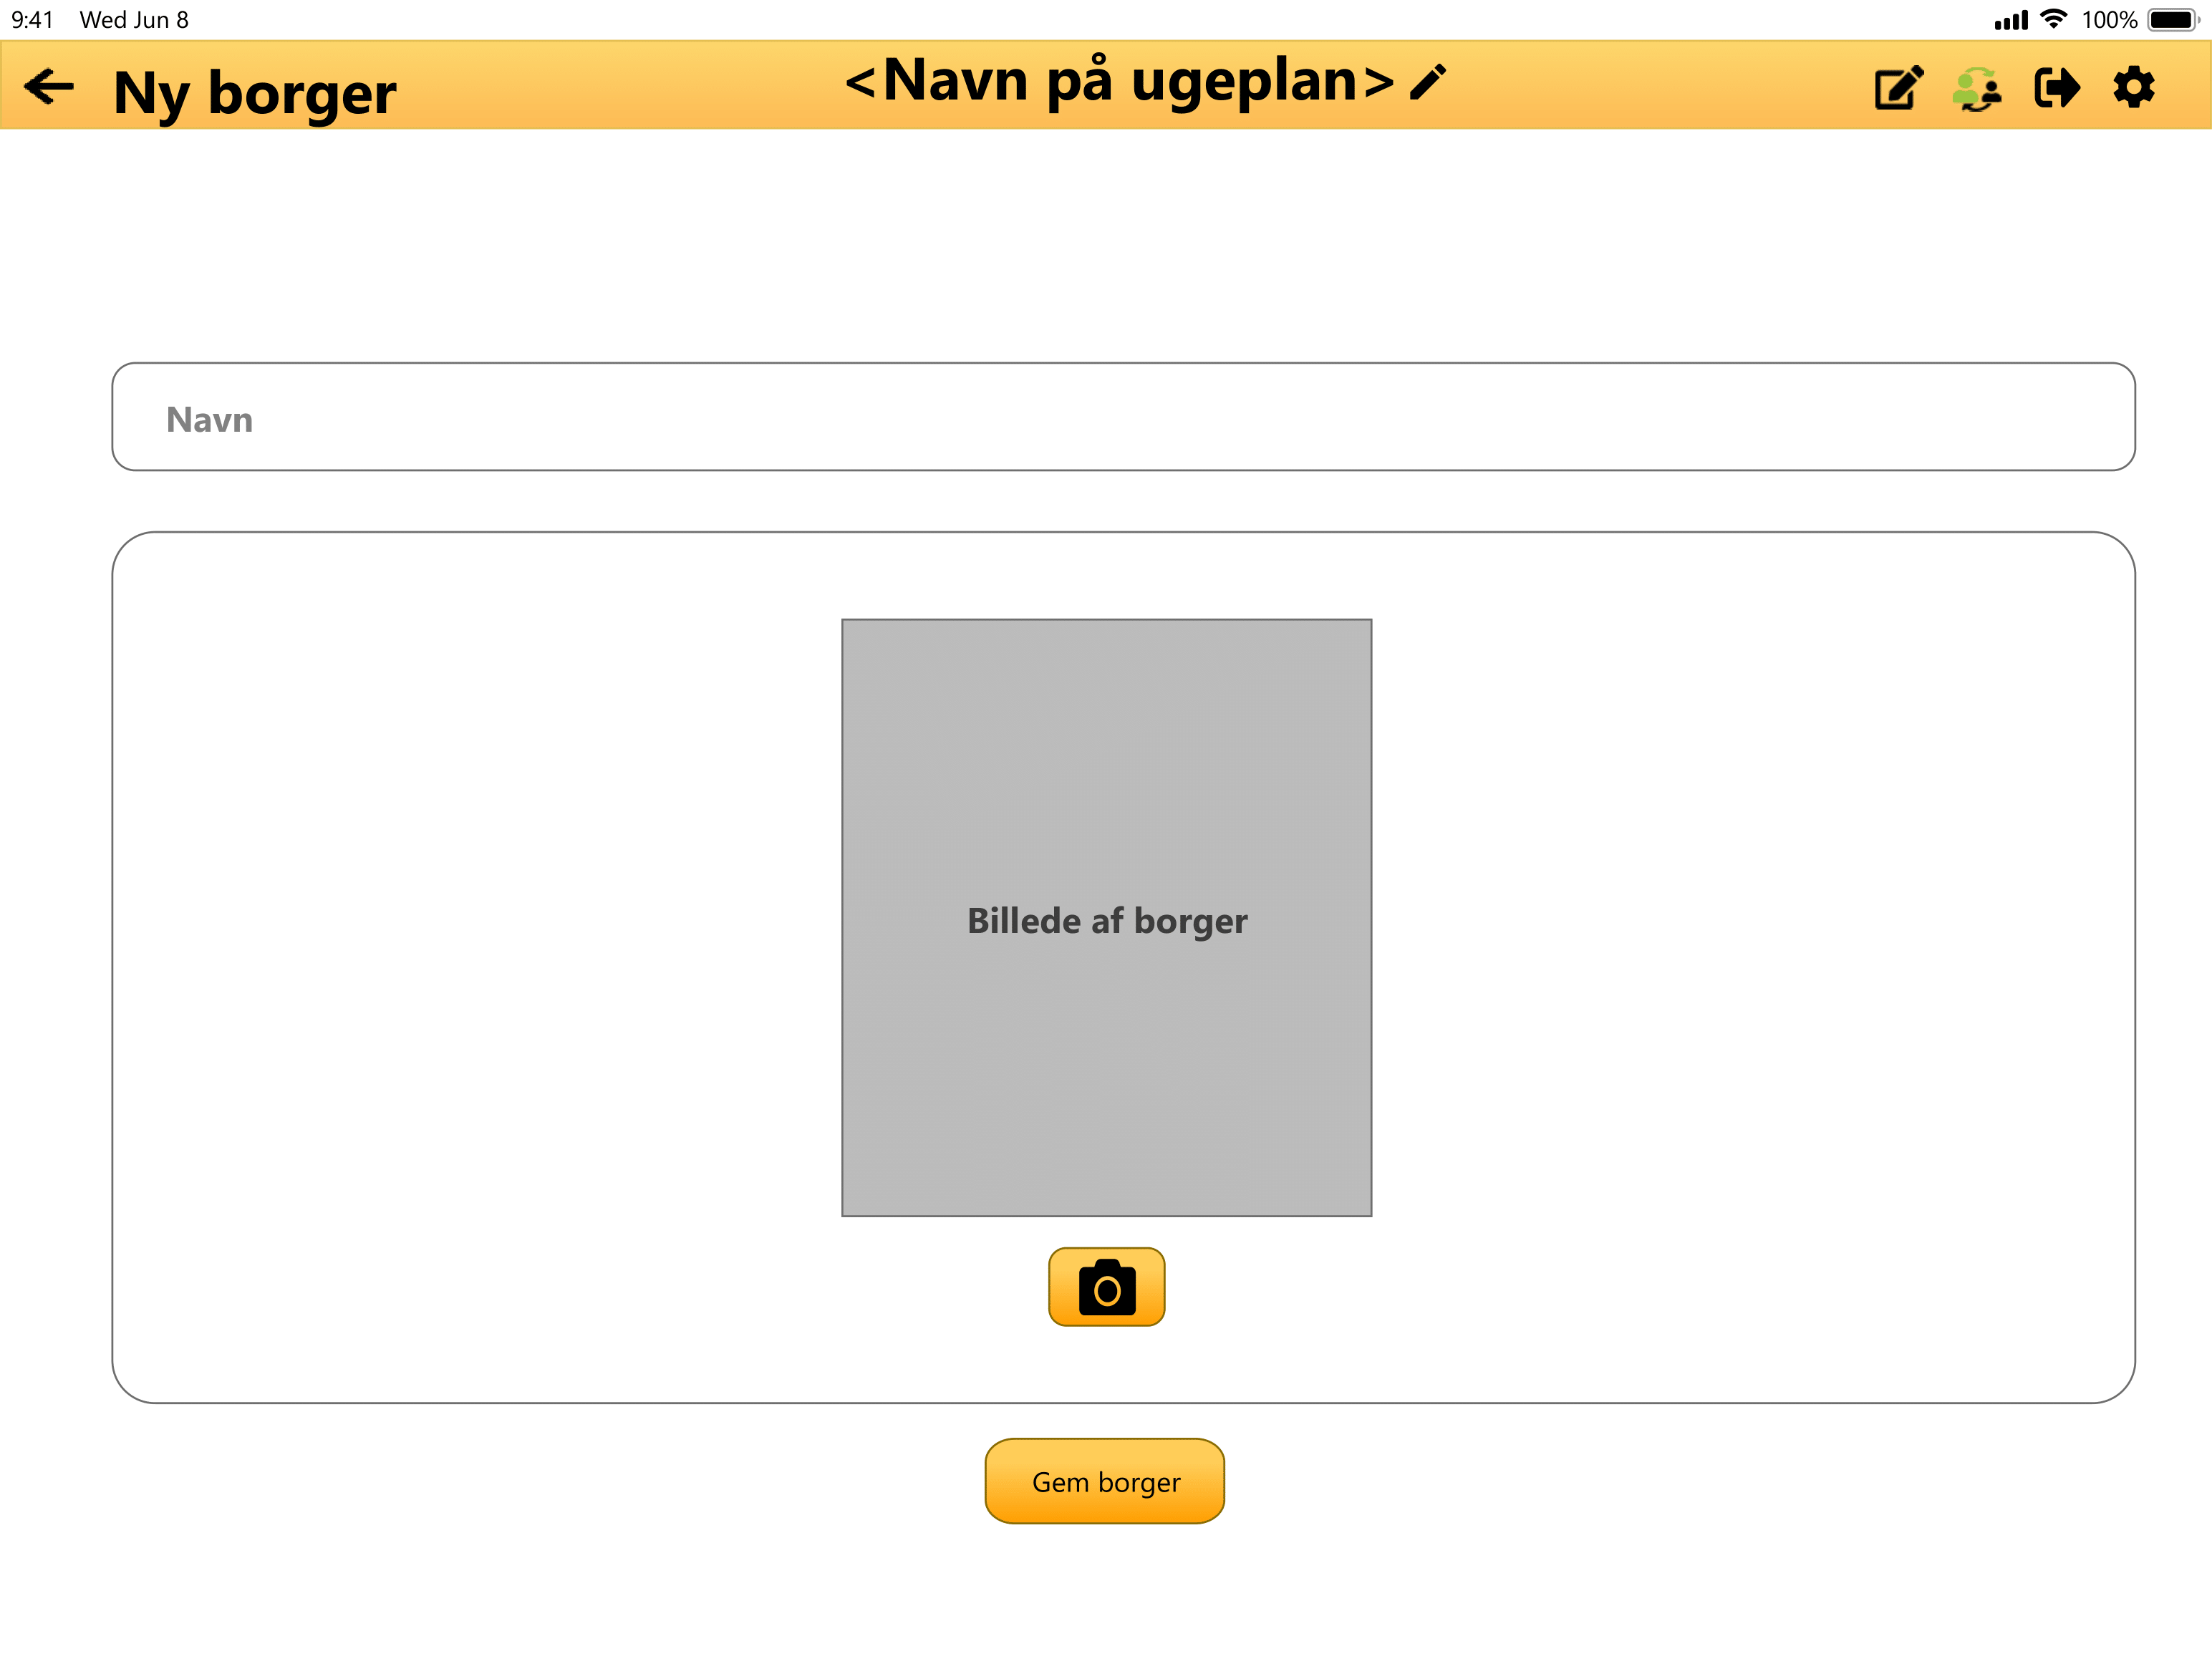
\includegraphics[width=1\linewidth, height=5cm]{add_citizen_2.png}
    \caption{The screen where a new citizen can be created}
    \label{subfig:add_citizen_2}
    \end{subfigure} 
    \caption{The prototypes for adding citizens.}
    \label{fig:add_citizen}
\end{figure}

\subsection{Edit citizens}
The guardians also needed to be able to edit their citizens, as the citizen could have changed class or be needing a new picture. 
\autoref{subfig:edit_citizen_1} is the settings screen where the guardian can change the currently selected citizen's information. 
\autoref{subfig:edit_citizen_2} shows the screen for changing the selected citizen's information.
This screen should show the citizen's current name, picture and class.
\begin{figure}[H]
    \begin{subfigure}{0.5\textwidth}
    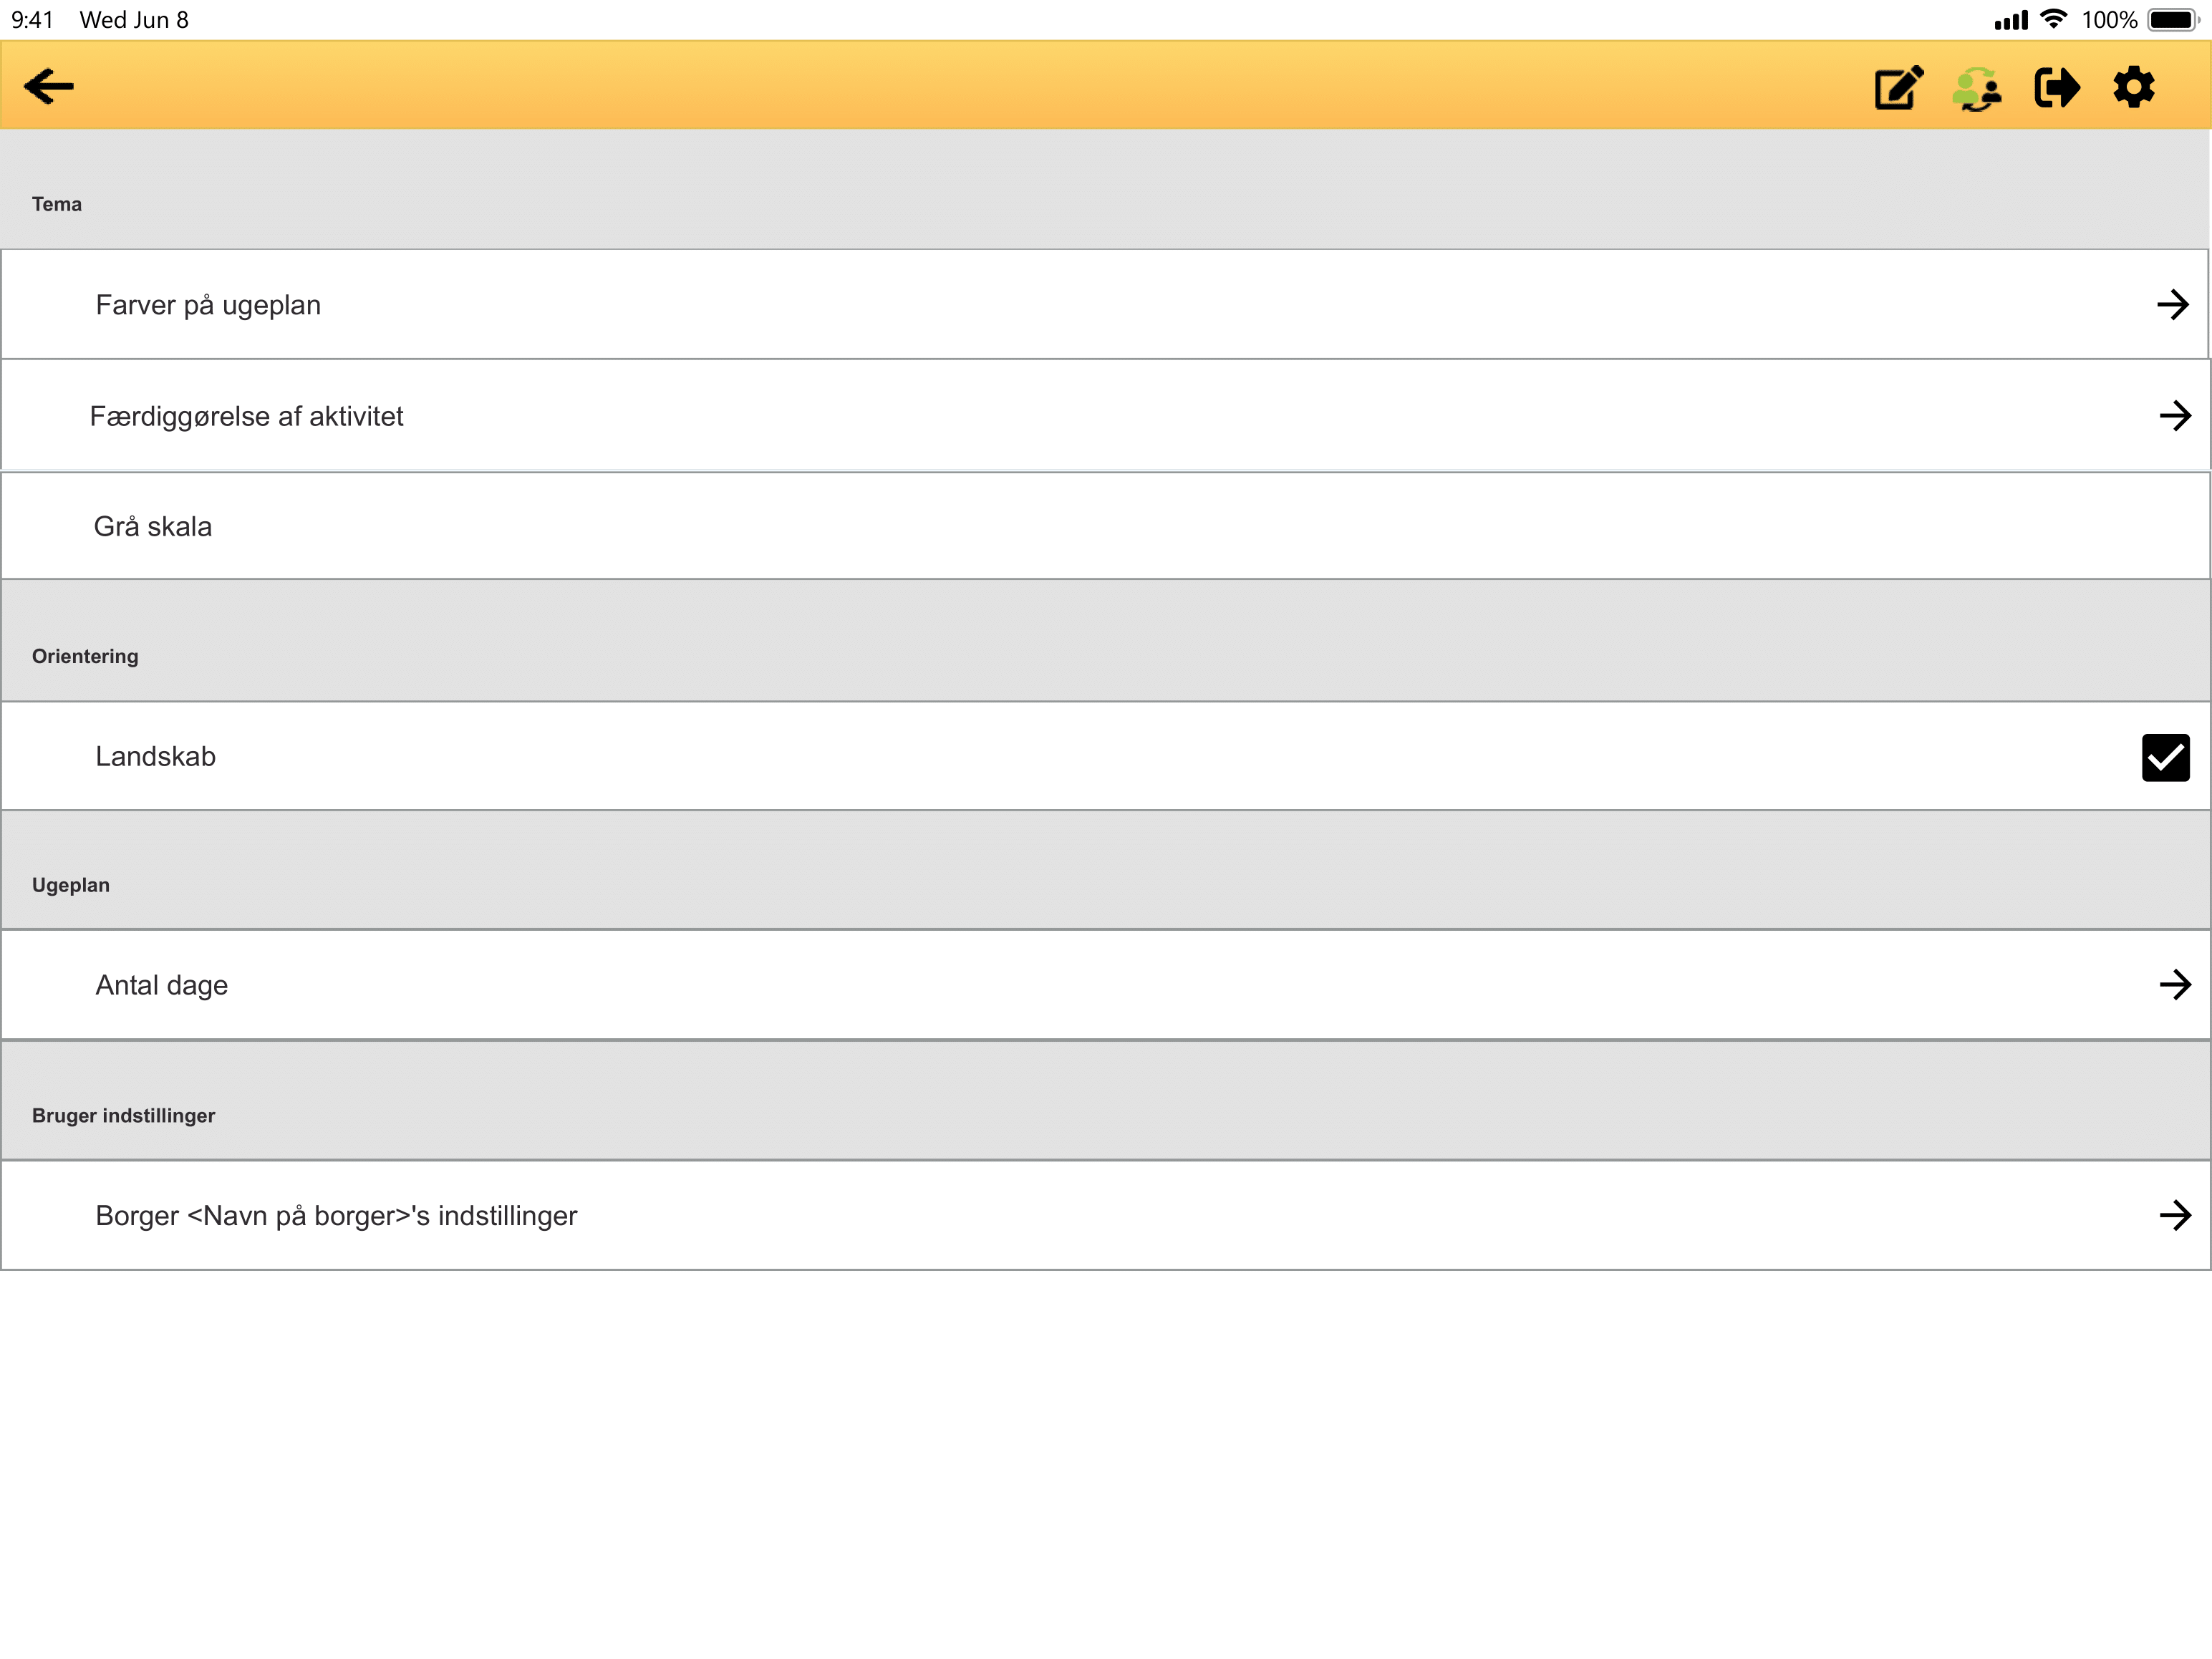
\includegraphics[width=1\linewidth, height=5cm]{edit_citizen_1.png}
    \caption{Settings screen where the guardian can go to the citizens edit screen}
    \label{subfig:edit_citizen_1}
    \end{subfigure}
    \begin{subfigure}{0.5\textwidth}
        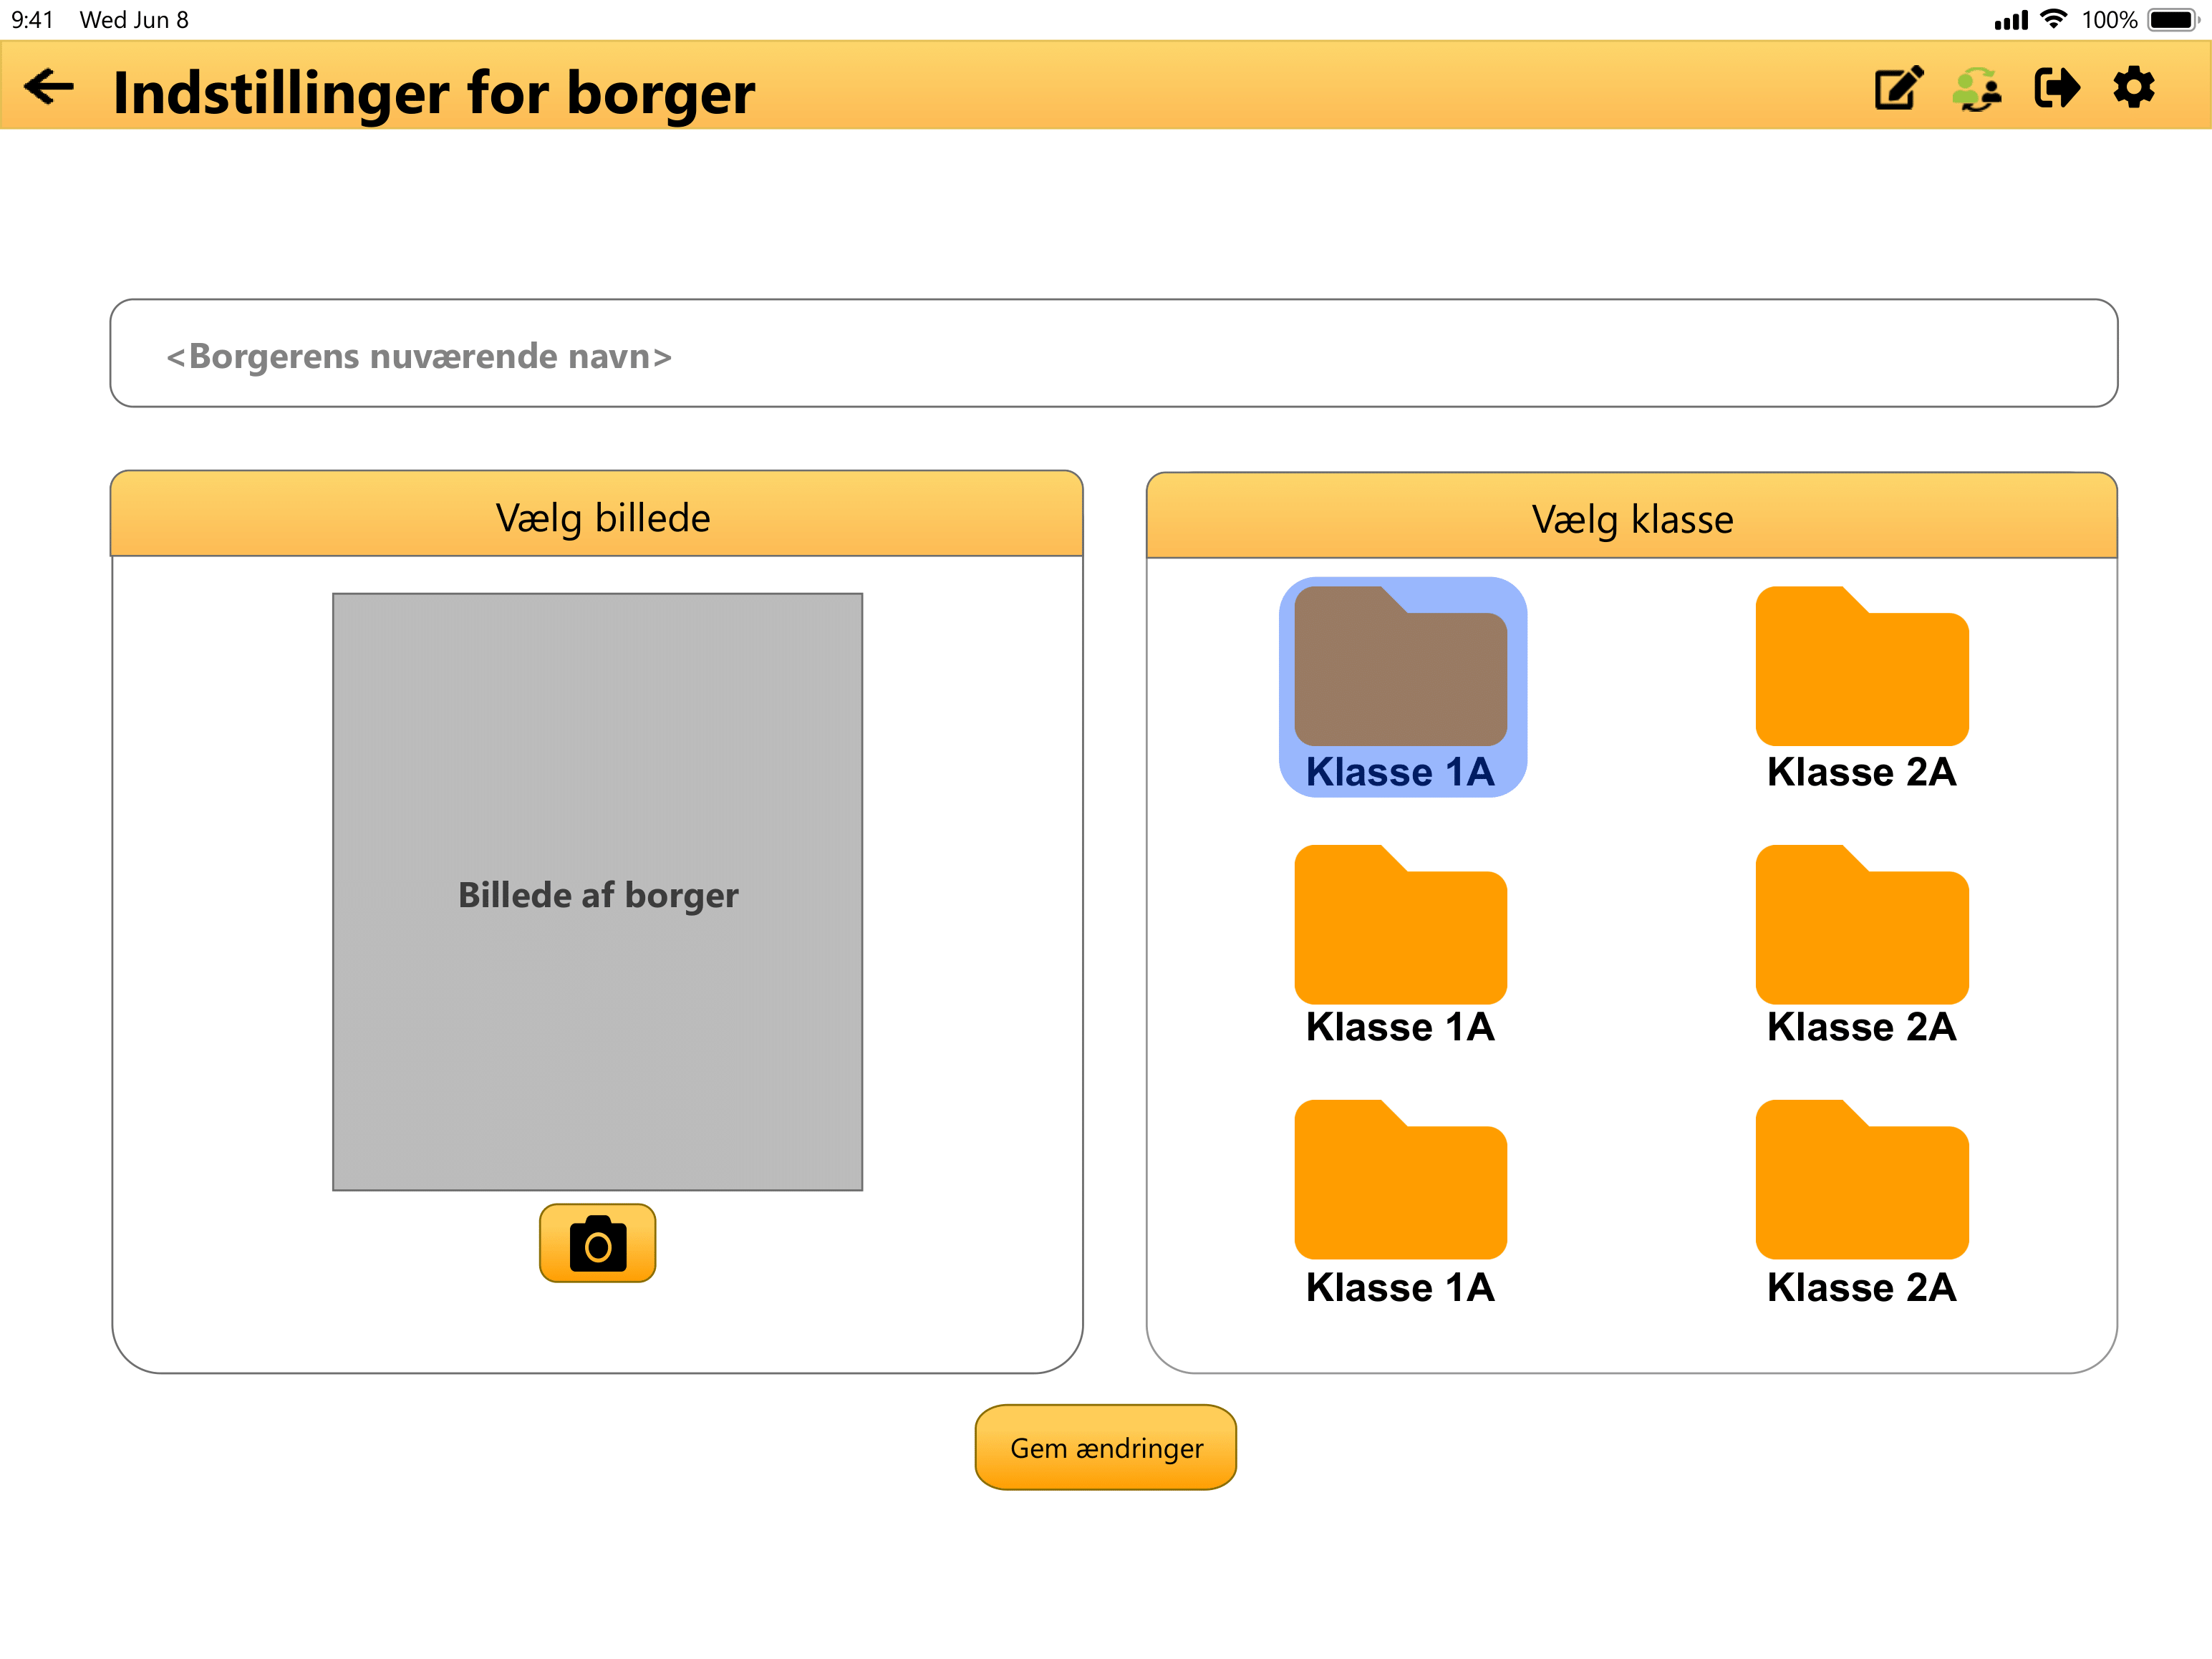
\includegraphics[width=1\linewidth, height=5cm]{edit_citizen_2.png}
    \caption{Edit citizen screen where name, picture and class can be changed}
    \label{subfig:edit_citizen_2}
    \end{subfigure} 
    \caption{The prototypes for editing citizen information.}
    \label{fig:edit_citizen}
\end{figure}
